\documentclass[10pt]{beamer}

\newcommand{\cl}{\mathrm{Cl^-}}
\newcommand{\br}{\mathrm{Br^-}}
\newcommand{\na}{\mathrm{Na^+}}
\newcommand{\h}{\mathrm{H^+}}
\newcommand{\ka}{\mathrm{K^+}}
\newcommand{\oh}{\mathrm{OH^-}}
\newcommand{\ca}{\mathrm{Ca^{2+}}}
\newcommand{\mg}{\mathrm{Mg^{2+}}}
\newcommand{\so}{\mathrm{SO_4^{2-}}}
\newcommand{\cs}{c_{\mathrm{s}}}
\newcommand{\gel}{^{gel}}
\newcommand{\Vgel}{V\gel}
\newcommand{\NA}{N_{\mathrm{A^-}}}
\newcommand{\pK}{\mathrm{p}K}
\newcommand{\pH}{\mathrm{pH}}
\newcommand{\cp}{c_\mathrm{p}}
\newcommand{\muna}{\mu_\mathrm{Na^+}}
\newcommand{\mucl}{\mu_\mathrm{Cl^-}}
\newcommand{\muca}{\mu_\mathrm{Ca^{2+}}}
\newcommand{\muh}{\mu_\mathrm{H^+}}
\newcommand{\mua}{\mu_\mathrm{A^-}}
\newcommand{\muha}{\mu_\mathrm{HA}}
\newcommand{\muoh}{\mu_\mathrm{OH}}
\newcommand{\cna}{c_\mathrm{Na^+}}
\newcommand{\ccl}{c_\mathrm{Cl^-}}
\newcommand{\cca}{c_\mathrm{Ca^{2+}}}
\newcommand{\ch}{c_\mathrm{H^+}}

\newcommand{\nna}{N_\mathrm{Na^+}}
\newcommand{\ncl}{N_\mathrm{Cl^-}}
\newcommand{\nca}{N_\mathrm{Ca^{2+}}}

\newcommand{\kT}{kT}
\usepackage{subfig}
\usetheme[progressbar=frametitle]{metropolis}
\usepackage{appendixnumberbeamer}

\usepackage{booktabs}
\usepackage[scale=2]{ccicons}

\usepackage{pgfplots}
\usepgfplotslibrary{dateplot}

\usepackage{xspace}
\newcommand{\themename}{\textbf{\textsc{metropolis}}\xspace}

\title{Water desalination using polyelectrolyte hydrogel.  }
\subtitle{Gibbs ensemble modelling.}
% \date{\today}
\author{Oleg V. Rud}
\institute{Department of Physical and Macromolecular Chemistry, Faculty of Science, Charles University in Prague, Hlavova 8, Praha 2 128 00, Czech Republic
\\
\\
Institute of Macromolecular Compounds of Russian Academy of Sciences, 199004, Bolshoy pr. 31, Saint-Petersburg, Russia
}

% \titlegraphic{\hfill
\includegraphics[height=1.5cm]{figures/cuni_logo.png}}

\begin{document}

\maketitle

%\begin{frame}{Table of contents}
%  \setbeamertemplate{section in toc}[sections numbered]
%  \tableofcontents%[hideallsubsections]
%\end{frame}

\section[Intro]{Introduction}
\begin{frame}[fragile]{Introduction. Desalination.}
\begin{enumerate}
\item Distillation
\item Reverse osmosis
\item Forward osmosis
\end{enumerate}
\end{frame}
\begin{frame}[fragile]{Introduction. Forward osmsis.}

\begin{enumerate}
	\item Hydrogels for desalination
	\item Forward osmosis
	\item Various stimuli: thermo-, pH-, electric-, magnetic-, light-indused gel shrinkage
\end{enumerate}
\begin{figure}[t]
	{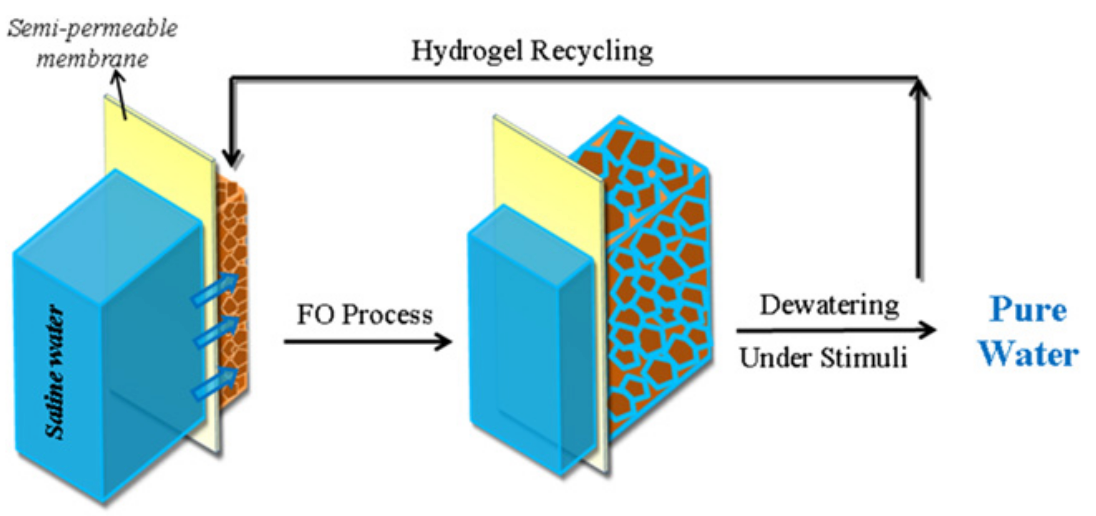
\includegraphics[width=\columnwidth]{{figures/FO}.png}}
\end{figure}
\end{frame}

%%%%%%%%%%%%%%%%%%%%%%%%%%%%%%%%%%%%%%%%%%%%%%%%%%%%%%%%%%%
\begin{frame}[fragile]{Introduction. Manfred Wilhelm experiment}
	\begin{columns}[T,onlytextwidth]% COLUMNS
		\column{0.4\textwidth}
			\begin{figure}[t]
				{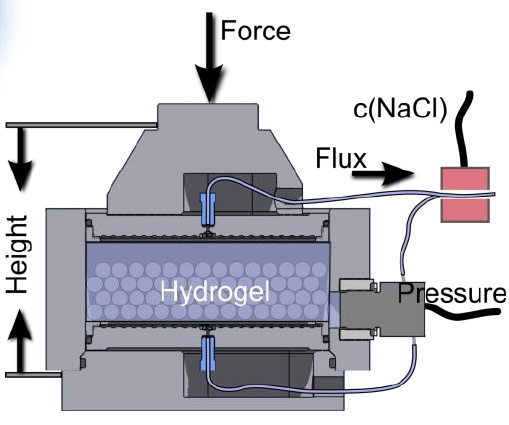
\includegraphics[width=0.9\columnwidth]{{figures/exp}.png}}
			\end{figure}

		\column{0.6\textwidth}
			\begin{figure}[t]
				{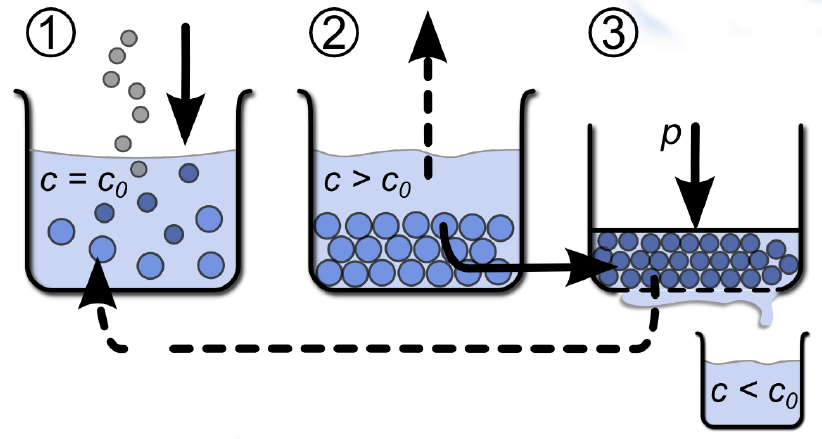
\includegraphics[width=0.9\columnwidth]{{figures/scheme}.png}}
			\end{figure}
	\end{columns}% COLUMNS
		
		
		
	{\scriptsize Fengler, C., Arens, L., Horn, H., Wilhelm, M. (2020). {\bf Desalination of Seawater Using Cationic Poly(acrylamide) Hydrogels and Mechanical Forces for Separation.} Macromolecular Materials and Engineering\\
	Yu, C., Wang, Y., Lang, X., Fan, S. (2016). {\bf A Method for Seawater Desalination via Squeezing Ionic Hydrogels.} Environmental Science and Technology}
\end{frame}
%%%%%%%%%%%%%%%%%%%%%%%%%%%%%%%%%%%%%%%%%%%%%%%%%%%%%%%%%%%

\section{The model of a polyelectrolyte gel.}
%%%%%%%%%%%%%%%%%%%%%%%%%%%%%%%%%%%%%%%%%%%%%%%%%%%%%%%%%%%
\begin{frame}[fragile]{Model of the gel}
  \begin{columns}[T,onlytextwidth]% COLUMNS
    \column{0.35\textwidth}
\begin{figure}
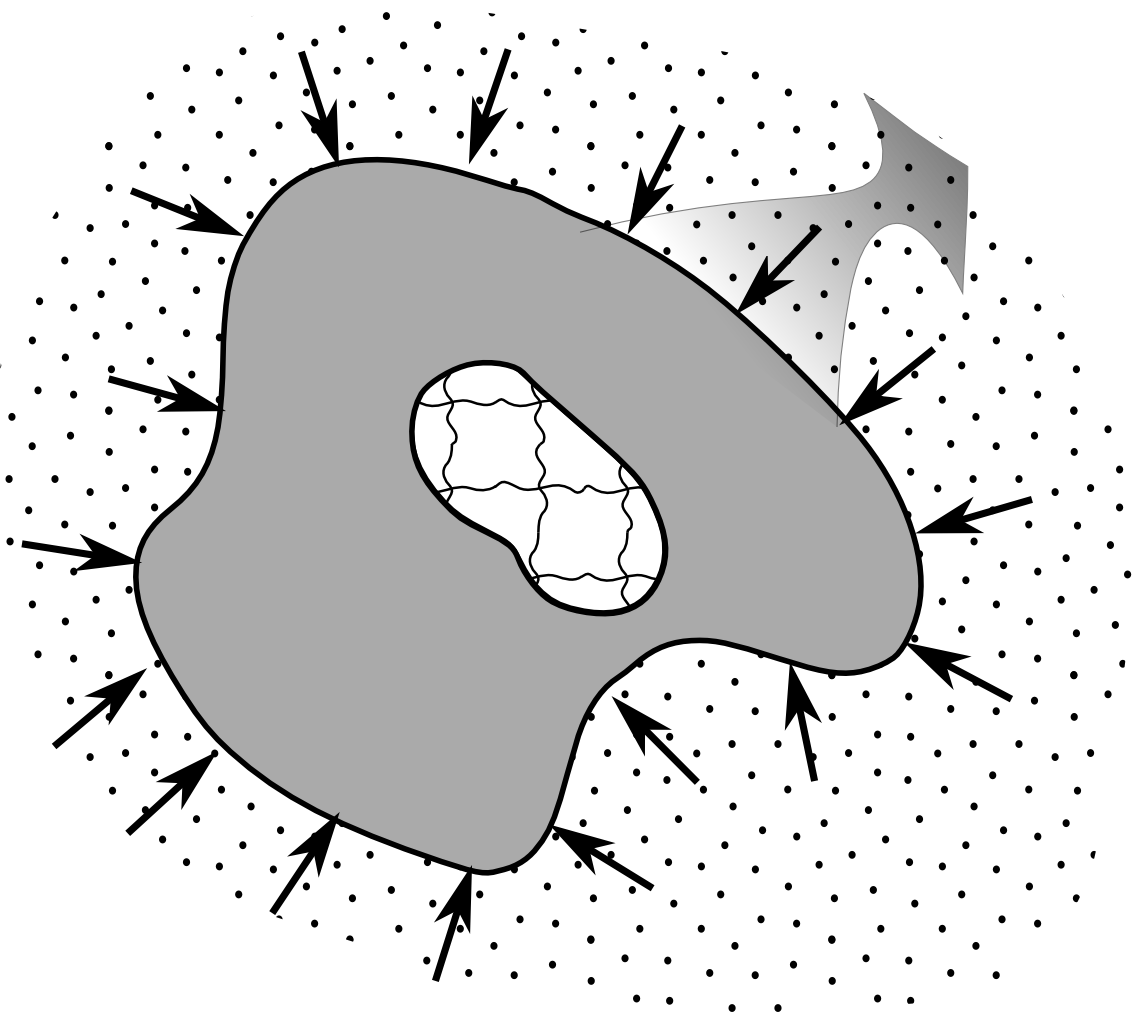
\includegraphics[height=4.5cm]{figures/gel_donnan.png}
\end{figure}   
  
  \column{0.55\textwidth}
  
\begin{itemize}
\item The gel is a particle of mAcro size 
\item In aqueous solution
\item Infinite network of polymer chains
\item Each bead is charged
\end{itemize}


  \end{columns}% COLUMNS
\begin{itemize}
\item The gel itself is a membrane
\item Donnan equilibrium
$c_s^2 = c^{in}_{Na}\cdot c^{in}_{Cl}$
\item The compression of hydrogel  affects the ionic composition of supernatant
\end{itemize}
  
\end{frame}

%%%%%%%%%%%%%%%%%%%%%%%%%%%%%%%%%%%%%%%%%%%%%%%%%%%%%%%%%%%


%%%%%%%%%%%%%%%%%%%%%%%%%%%%%%%%%%%%%%%%%%%%%%%%%%%%%%%%%%%
\begin{frame}[fragile]{Model of the gel. Two ensembles.}

	\begin{columns}[T,onlytextwidth]% COLUMNS
		\column{0.5\textwidth}
			\begin{figure}[t]
				{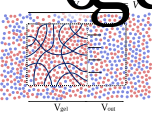
\includegraphics[width=0.9\columnwidth]{{figures/gc}.pdf}}
			\end{figure}
			\centering Open system \\(grand-cannonical ensemble)
		\column{0.5\textwidth}
			\begin{figure}[t]
				{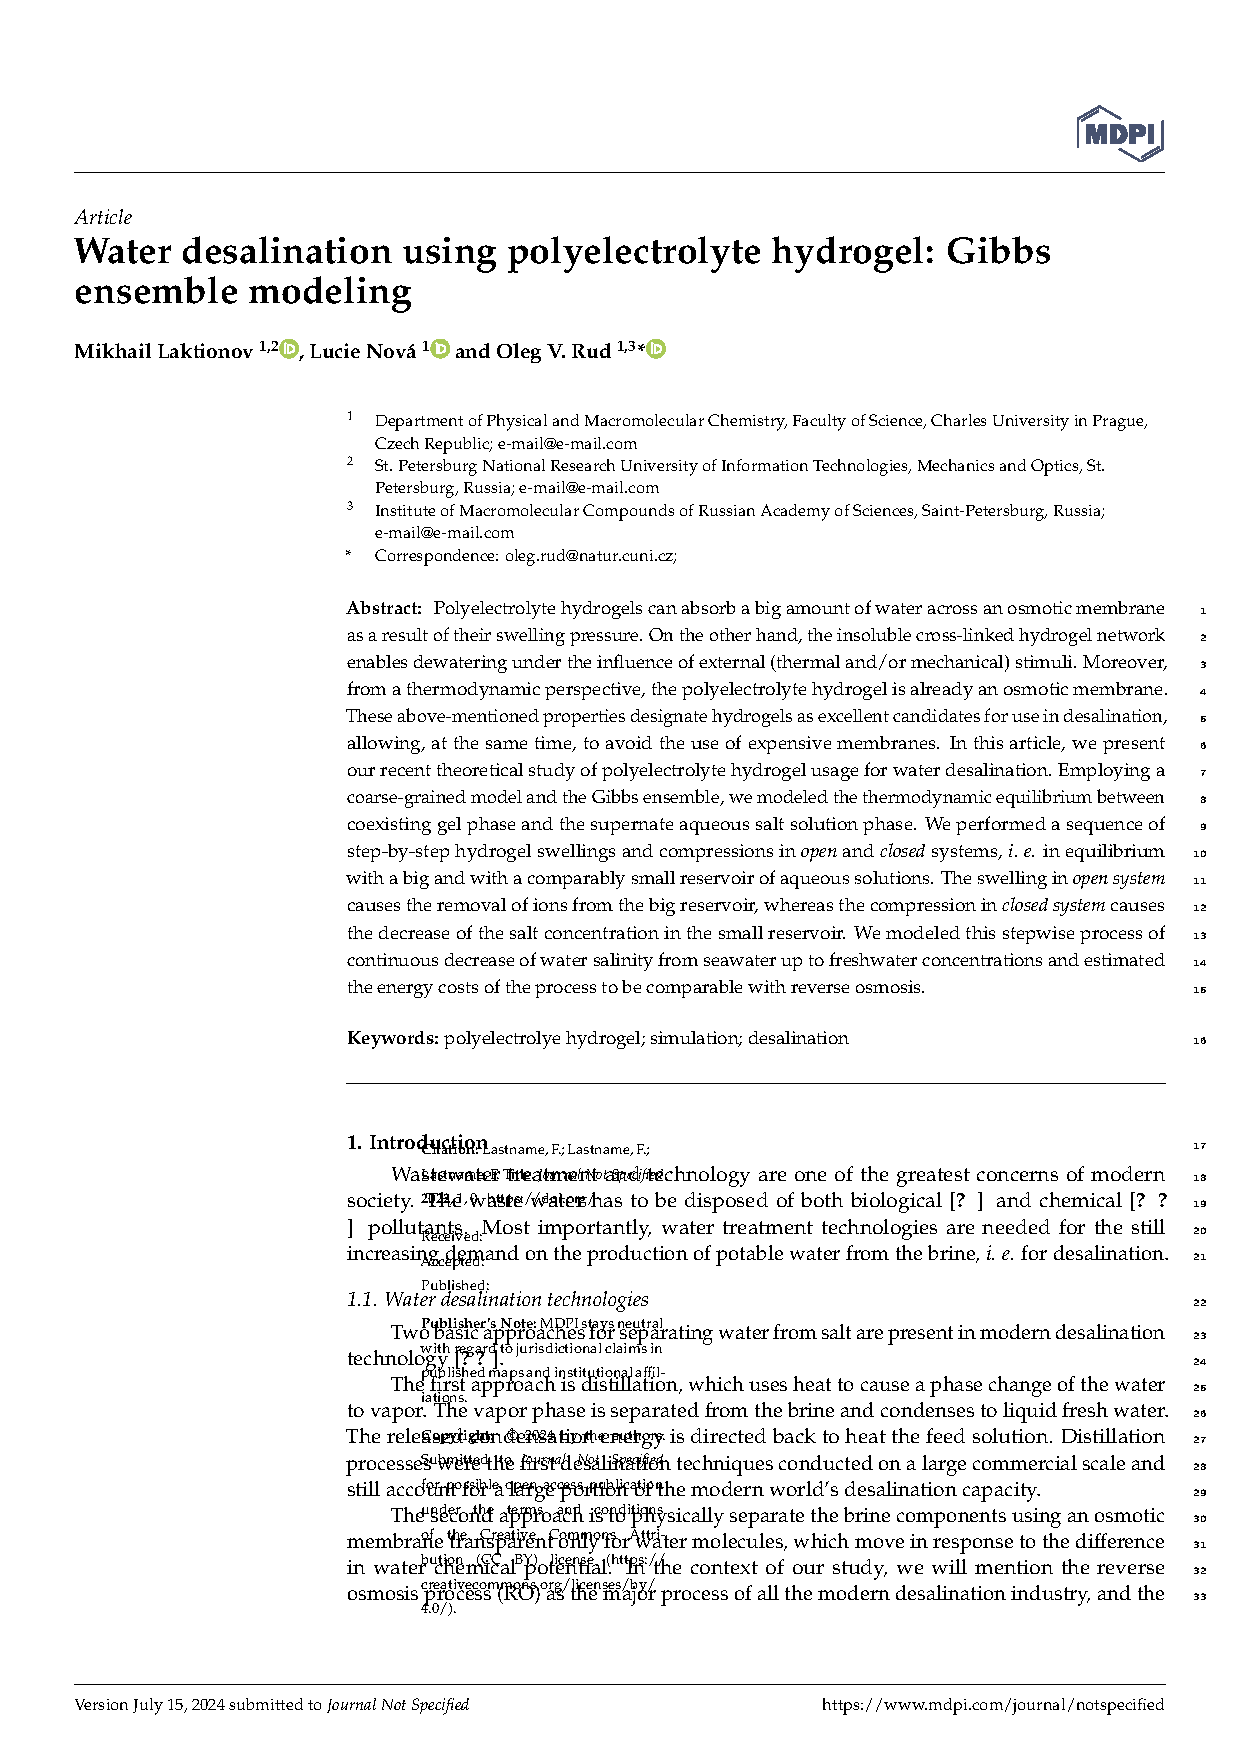
\includegraphics[width=0.9\columnwidth]{{figures/gibbs}.pdf}}
			\end{figure}
			\centering Closed system \\(Gibbs ensemble)
	\end{columns}% COLUMNS
	
\end{frame}
%%%%%%%%%%%%%%%%%%%%%%%%%%%%%%%%%%%%%%%%%%%%%%%%%%%%%%%%%%%

\subsection{Grand-cannonical ensemble.}
%%%%%%%%%%%%%%%%%%%%%%%%%%%%%%%%%%%%%%%%%%%%%%%%%%%%%%%%%%%


\begin{frame}{Grand-cannonical ensemble.}
	\begin{columns}[T,onlytextwidth]% COLUMNS
	\column{0.5\textwidth}
	\column{0.5\textwidth}
	The free energy of the grand-canonical ensemble exchanging ion pair with the bath
	\begin{equation*}
		\boxed{
		\Omega=E-TS+\mu N}
	\end{equation*}
	The entropy $S$ expands via Boltzmann formula
		\begin{equation*}
			S=k_{B}\ln\frac{V^{N}}{N!}\label{eq:entropy}
		\end{equation*}
	\end{columns}% COLUMNS		
	The change of free energy associated with a single particle exchange is 
	\begin{equation*}
		\boxed{
		\Delta\Omega=k_BT\xi\ln V \left(N+\theta(\xi)\right)+\xi\mu+\Delta E\label{eq: DeltaG GC}}
	\end{equation*}
	{\tt accept if $\mathcal{R}^{\xi}<e^{\Delta\Omega/k_BT}$}
\end{frame}
%%%%%%%%%%%%%%%%%%%%%%%%%%%%%%%%%%%%%%%%%%%%%%%%%%%%%%%%%%%



\subsection{Gibbs ensemble.}
%%%%%%%%%%%%%%%%%%%%%%%%%%%%%%%%%%%%%%%%%%%%%%%%%%%%%%%%%%%
\begin{frame}{Gibbs ensemble.}
	\begin{columns}[T,onlytextwidth]% COLUMNS
		\column{0.5\textwidth}
		\begin{figure}[t]
			{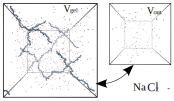
\includegraphics[width=0.9\columnwidth]{{figures/simgibbs}.pdf}}
		\end{figure}
		\column{0.5\textwidth}
			The free energy of the grand-canonical ensemble for single particle type
	\begin{equation*}
		\boxed{
		\Omega=E_1+E_2-TS}
	\end{equation*}
	
	\begin{equation}
		S=k_B \ln \frac{V_1^{N_1}}{N_1!}\frac{V_2^{N_2}}{N_2!}
	\end{equation}
	\end{columns}% COLUMNS		
	The change of free energy associated with a single particle exchange is 
	\begin{equation*}
		\boxed{
		\Delta\Omega=k_BT\xi \ln\left(\frac{V_1}{V_2}\frac{N_2+\theta(-\xi)}{N_1+\theta(\xi)}\right)+\Delta E_1 +\Delta E_2\label{eq: DeltaG GC}}
	\end{equation*}
	{\tt accept if $\mathcal{R}^{\xi}<e^{\Delta\Omega/k_BT}$}
			
\end{frame}
%%%%%%%%%%%%%%%%%%%%%%%%%%%%%%%%%%%%%%%%%%%%%%%%%%%%%%%%%%%

\subsection{Langevin dynamics.}
%%%%%%%%%%%%%%%%%%%%%%%%%%%%%%%%%%%%%%%%%%%%%%%%%%%%%%%%%%%
\begin{frame}{Langevin dynamics. }
	\begin{columns}[T,onlytextwidth]% COLUMNS
		\column{0.4\textwidth}
			\begin{figure}
				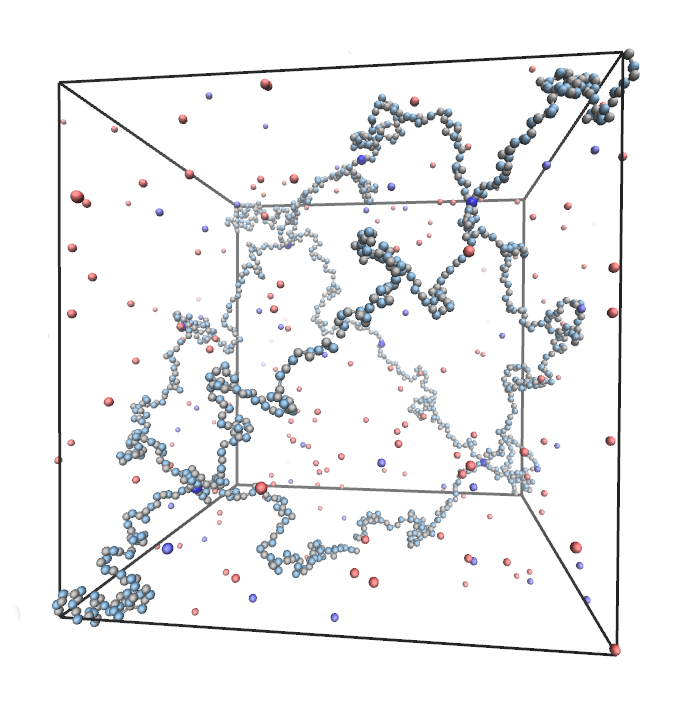
\includegraphics[height=4.5cm]{figures/snapshot_cut.png}
				\caption{The snapshot of the hydrogel model for Langevin dynamics}
			\end{figure}   
		\column{0.01\textwidth}
		\column{0.6\textwidth}

		\begin{itemize}
			\item 
				Diamond network of point particles
			\item
				Lennard--Jones interaction
		\end{itemize}
		\begin{equation*}
			V_{LJ}(r) = 
			\begin{cases}
				4\varepsilon\left(\left(\frac{\sigma}{r-r_c}\right)^{12}-\left(\frac{\sigma}{r-r_c}\right)^{6}\right) & ,\ r<r_{c}\\
				0 & ,\ r>r_{c}
			\end{cases}
		\end{equation*}
		\begin{itemize}
			\item FENE potential
			\begin{equation*}
				V_{FENE}(r)=-\frac{1}{2}\Theta\Delta r_{max}^{2}\ln\left[1-\left(\frac{r-r_{0}}{\Delta r_{max}}\right)^{2}\right]
			\end{equation*}
			\item
				Electrostatic interaction
				\begin{equation*}
					V_{EL}=l_{B}k_{B}T\cdot\frac{q_{1}q_{2}}{r}
				\end{equation*}

		\end{itemize}

	\end{columns} % COLUMNS
\end{frame}

\subsection{Grand-reaction ensemble.}

{
\usebackgroundtemplate{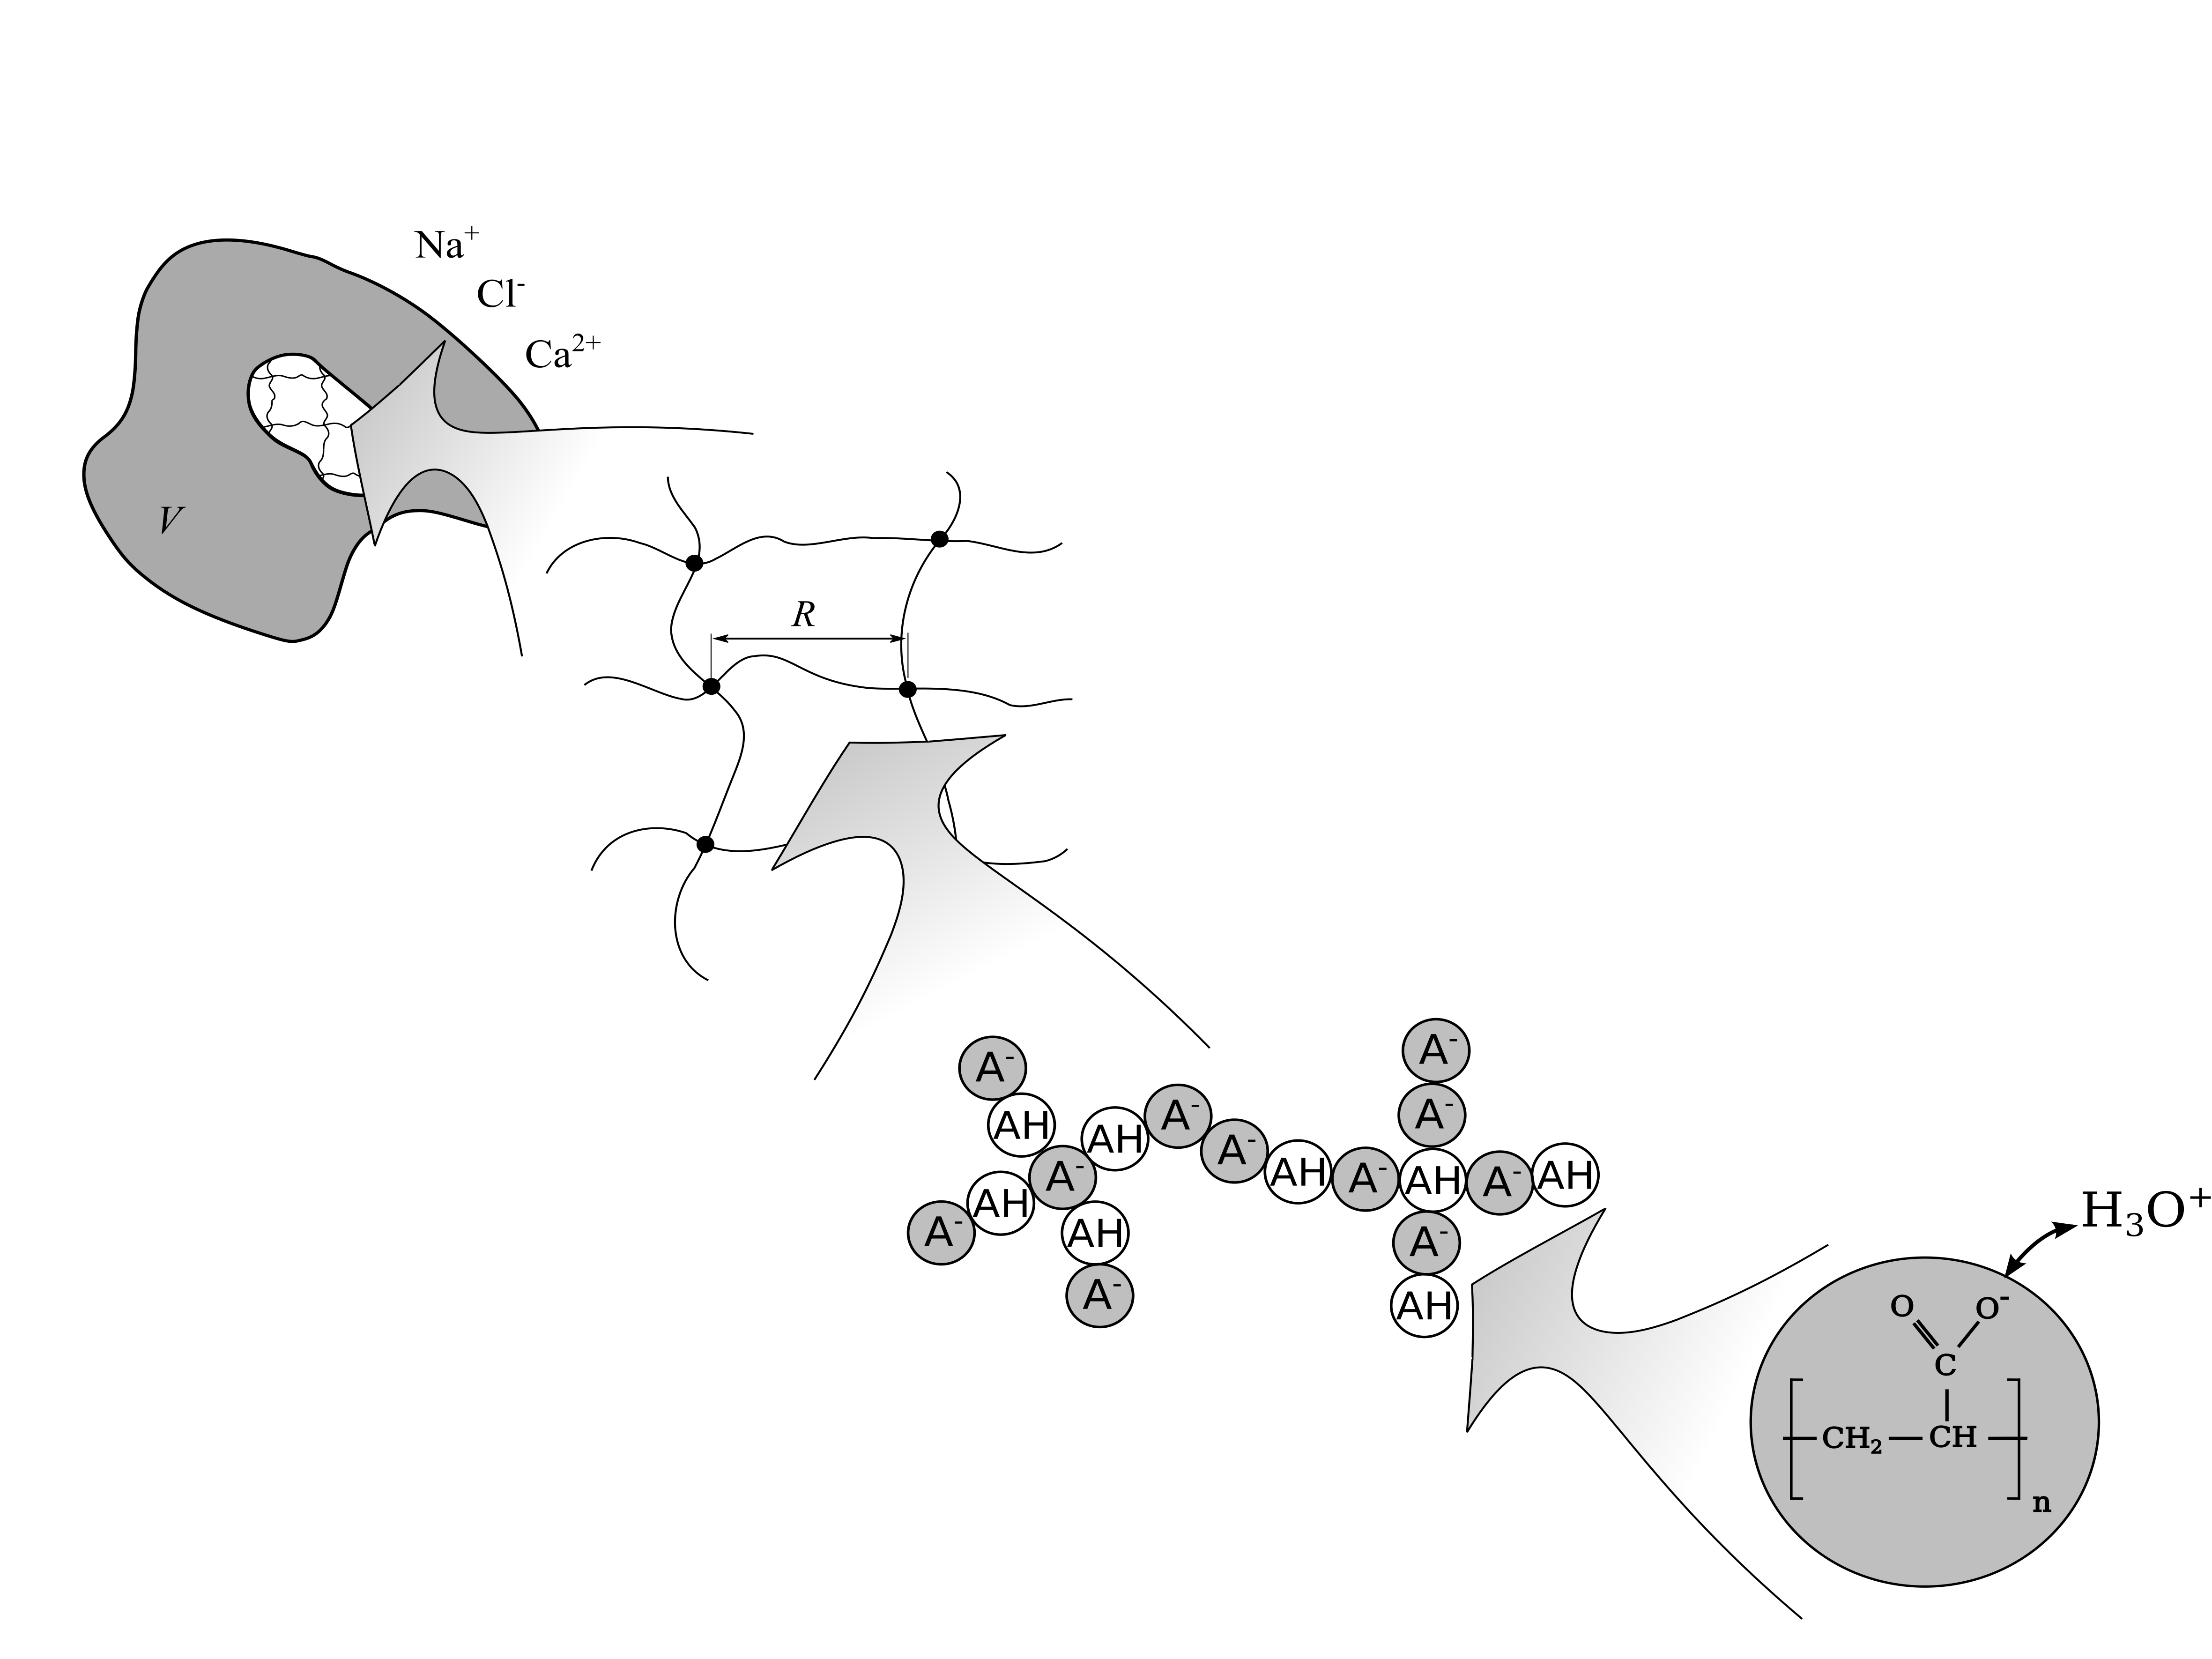
\includegraphics[width=\paperwidth]{figures/grand_reaction_model.png}}
\begin{frame}{Grand-reaction ensemble.}
\begin{columns}[T,onlytextwidth]% COLUMNS
\column{0.3\textwidth}
\vspace{4.5cm}
Ionization equilibrium in \textbf{reaction} ensemble
\begin{equation*}
	\boxed{
		\mathrm{pA^- + H_3O^+ \leftrightarrows pAH}
	}
\end{equation*}

\column{0.4\textwidth}
Constant salinity 
\begin{equation*}
\boxed{c_s = c_\mathrm{Cl}^- = c_\mathrm{Na}^+}
\end{equation*}
The simulation box freely 
exchanges ions with reservoir as in \textbf{grand cannonical} ensemble
\end{columns} % COLUMNS
\vspace{0.5cm}
{\scriptsize Landsgesell, J., Hebbeker, P., Rud, O., Lunkad, R., Košovan, P., \\ Holm, C. (2020). 
{\bf Grand-Reaction Method for Simulations of Ionization \\
Equilibria Coupled to Ion Partitioning. }
Macromolecules, 53(8), 3007–3020. }
\end{frame}
}

{

}

{

\begin{frame}{Grand-reaction ensemble.}

	\begin{columns}[T,onlytextwidth]% COLUMNS
		\column{0.5\textwidth}
			\begin{figure}
				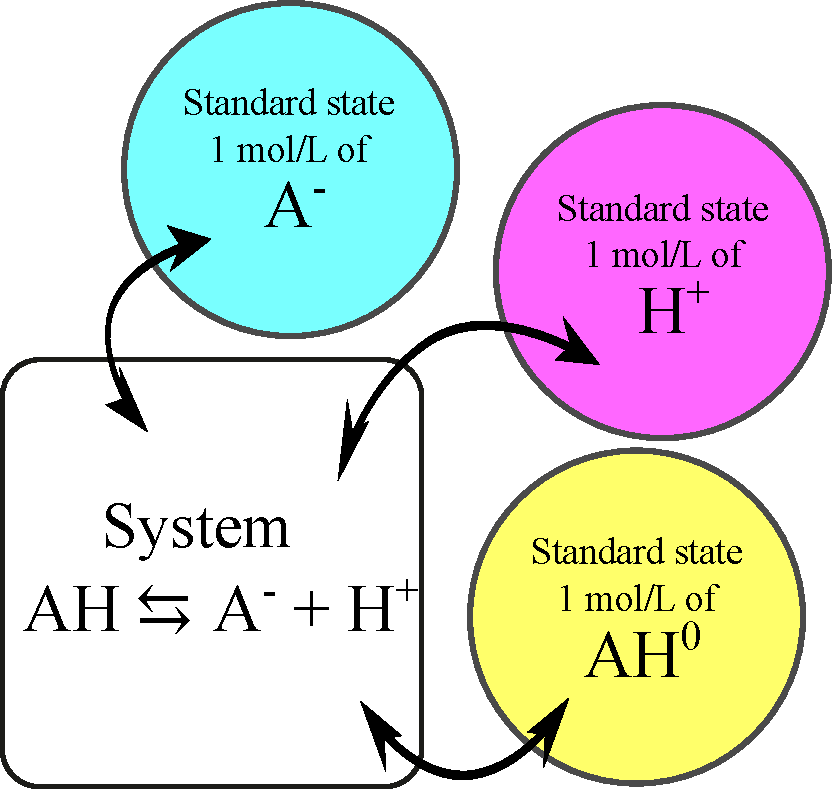
\includegraphics[height=4.cm]{figures/standard_states.pdf}
			\end{figure} 
		\column{0.5\textwidth}	
			\textbf{Reaction ensemble}\\ 
			\vspace{1cm}
			The reaction of an acidic unit 
			\begin{equation*}
				\mathrm{HA}\stackrel{K}{\leftrightarrows}\mathrm{A^-}+\mathrm{H^+}\label{eq: acid reaction}
			\end{equation*}
			\begin{equation*}
				\Omega=E-TS+\sum_i\left(\mu_i-\mu^\ominus_i\right) N_i\label{eq:Omega-RE}
			\end{equation*}
	\end{columns} % COLUMNS
	\vspace{1cm}
	Then the change of system free energy during a single reaction step
	\begin{equation*}
		\Delta\Omega=k_BT\ln\left(\prod_i V^{\nu_i\xi}\frac{N_i!}{\left(N_i+\nu_i\xi\right)!}\right)+
		\xi\left(\sum_i\nu_i\mu_i-\sum_i\nu_i\mu_i^\ominus\right)+\Delta E
		\label{eq: DeltaG RE one}
	\end{equation*}
	{\tt accept if $\mathcal{R}^{\xi}<e^{\Delta\Omega/k_BT}$}
\end{frame}
}


\begin{frame}{Grand-reaction ensemble.}
\begin{columns}[T,onlytextwidth]% COLUMNS
\column{0.7\textwidth}
\begin{equation*}\boxed{
\Delta\Omega=k_BT\ln\left(K^\xi\prod_i V^{\nu_i\xi}\frac{N_i!}{\left(N_i+\nu_i\xi\right)!}\right)+\Delta E}
\end{equation*}
\column{0.3\textwidth}
\begin{equation*}\boxed{
K = e^{-\sum_i\nu_i \mu_i^\ominus }} 
\end{equation*}
\end{columns} % COLUMNS

\vspace{0.6cm}
\begin{columns}[T,onlytextwidth]% COLUMNS
\column{0.5\textwidth}
	\begin{equation*}
		\mathrm{HA}\stackrel{K}{\leftrightarrows}\mathrm{A^-}+\mathrm{H^+} 
	\end{equation*}
	\begin{equation*}
		K= \mu_\h^\ominus+\mu_\mathrm{A^-}^\ominus - \mu_\mathrm{HA}^\ominus
	\end{equation*}
	\vspace{0.2cm}
\begin{equation*}
\emptyset \leftrightarrows  \na  +\cl
\end{equation*}
\begin{equation*}
K= \mu_\na+\mu_\cl
\end{equation*}
\vspace{0.2cm}
\begin{equation*}
\emptyset \leftrightarrows \ca + 2\cl
\end{equation*}
\begin{equation*}
K= 2\mu_\ca+\mu_\cl
\end{equation*}
\column{0.5\textwidth}
			\begin{figure}
				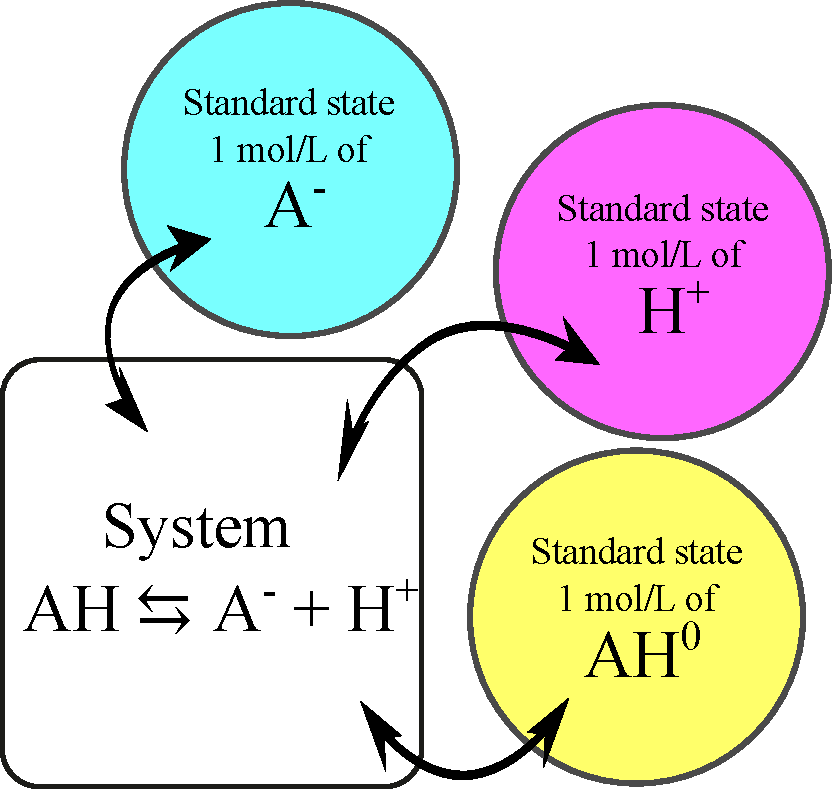
\includegraphics[height=4.cm]{figures/standard_states.pdf}
			\end{figure} 
\end{columns} % COLUMNS

\end{frame}







\begin{frame}{Simulation protocol.}
\begin{enumerate}
\item {\tt Choose randomly: LMD, RE, or EX.}	\vspace{0.5cm}
\item {\tt Simulate the chosen, collecting 50 samples of: }
	\vspace{0.3cm}
	\begin{columns}[T,onlytextwidth]% COLUMNS
		\column{0.3\textwidth}
			\fbox{\parbox{\textwidth}{LMD: pressure, $P$, and $\{R_e\}$}}
		\column{0.3\textwidth}
	       		\fbox{\parbox{\textwidth}{RE: number of ionized segments, $\NA$}}
      		\column{0.3\textwidth}
        		\fbox{\parbox{\textwidth}{EX: number of salt ions, $N_\na$ and $N_\cl$}}
	\end{columns} % COLUMNS
	\vspace{0.5cm}
    {\tt Check the autocorrelation of each samples array.\\
    Pearson coefficient must be < 0.2. }
	\vspace{0.5cm}
\item {\tt Repeat collecting at least 200 averages from each process}.
\end{enumerate}
\end{frame}

\section{Results}

\begin{frame}{Monovalent salt. Compression.}
	\begin{figure}[t]
		\subfloat[low salinity, $c_s = 0.007$ mol/l]
			{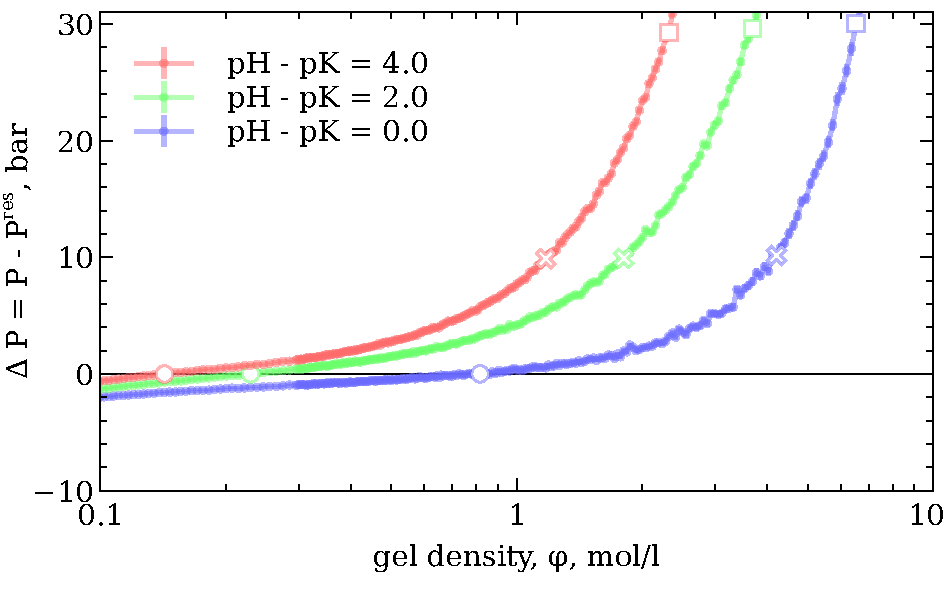
\includegraphics[width=0.5\columnwidth]{{figures/gel_pressure_log_density_cs0.006_N_Samples200}.pdf}}
			{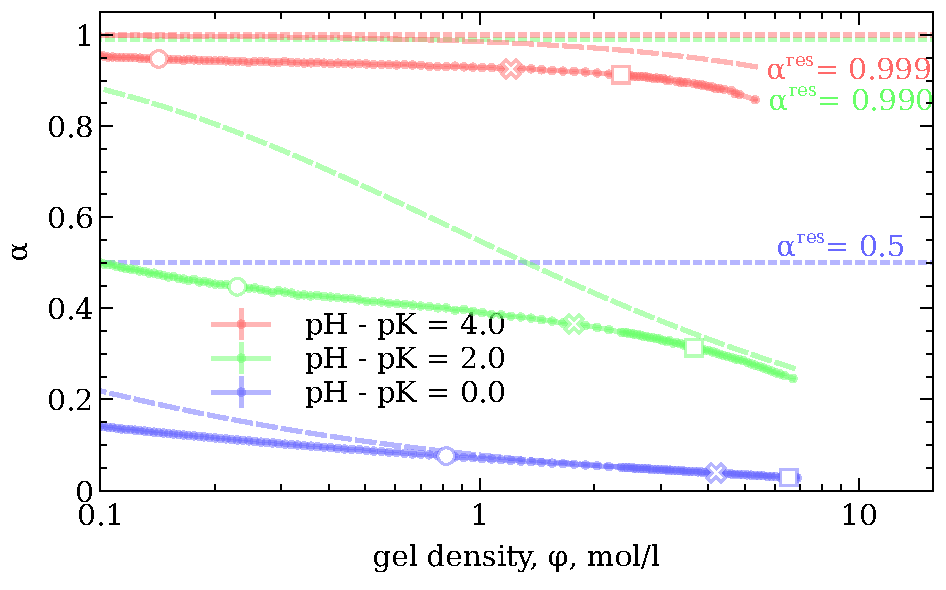
\includegraphics[width=0.5\columnwidth]{{figures/gel_alpha_log_density_cs0.006_N_Samples200}.pdf}}
		\subfloat[high salinity, $c_s = 0.209$ mol/l]
			{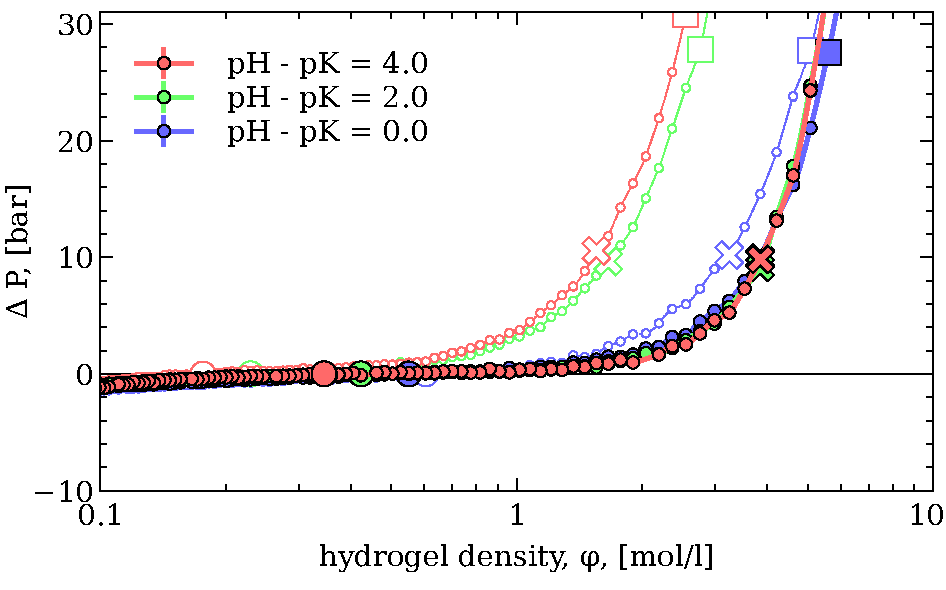
\includegraphics[width=0.5\columnwidth]{{figures/gel_pressure_log_density_cs0.15_N_Samples200}.pdf}}
			{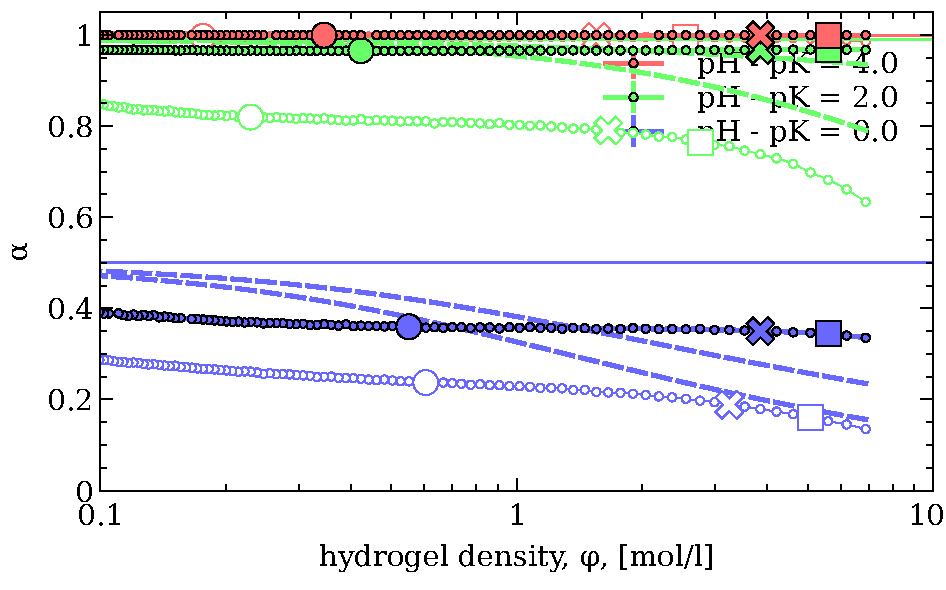
\includegraphics[width=0.5\columnwidth]{{figures/gel_alpha_log_density_cs0.15_N_Samples200}.pdf}}
	\end{figure}
\end{frame}

\begin{frame}{Monovalent salt. ``No electrostatics'' vs ``Mean field theory''.}
	\begin{equation*}
		\frac{\alpha}{1-\alpha}10^{\pK-\pH} =\sqrt{1+\left(\frac{\alpha\cp}{2\cs}\right)^{2}} - \frac{\alpha\cp}{2\cs}
	\end{equation*}
	Together with electroneutrality condition it translates to
	\begin{equation*}
		-\frac{{{\alpha}^{3}}{\cp}}{{\cs}}+
		{\alpha}^{2}\left(\frac{{\cp}}{{\cs}}+\Theta-\frac{1}{\Theta}\right)+
		\frac{2 \alpha}{\Theta}-\frac{1}{\Theta}=0
	\end{equation*}
	where $\Theta = 10^{\pK-\pH}$.
	\begin{figure}
		\subfloat[low salinity, $c_s = 0.007$ mol/l]
			{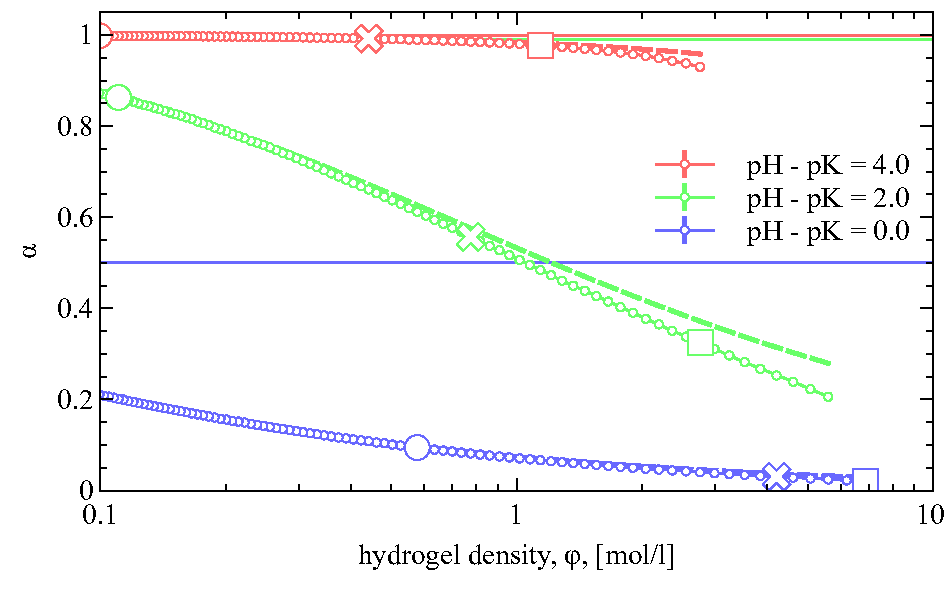
\includegraphics[width=0.47\columnwidth]{{figures/gel_alpha_log_density_lB0.0_cs0.006_N_Samples200}.pdf}}
\subfloat[high salinity, $c_s = 0.209$ mol/l]
			{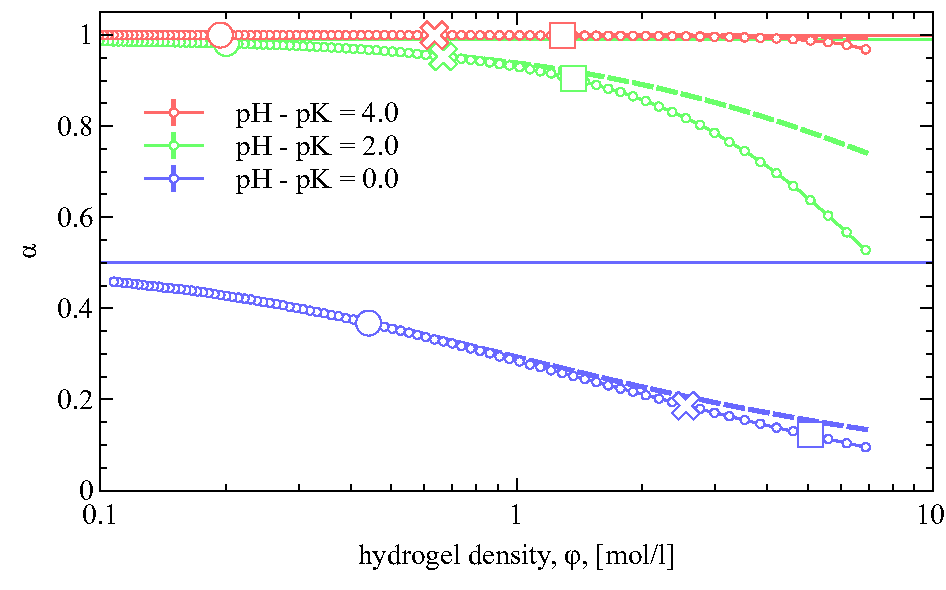
\includegraphics[width=0.47\columnwidth]{{figures/gel_alpha_log_density_lB0.0_cs0.15_N_Samples200}.pdf}}
	\end{figure}
\end{frame}



\begin{frame}{Monovalent salt. Desalination effect.}

	\begin{figure}[t]
		{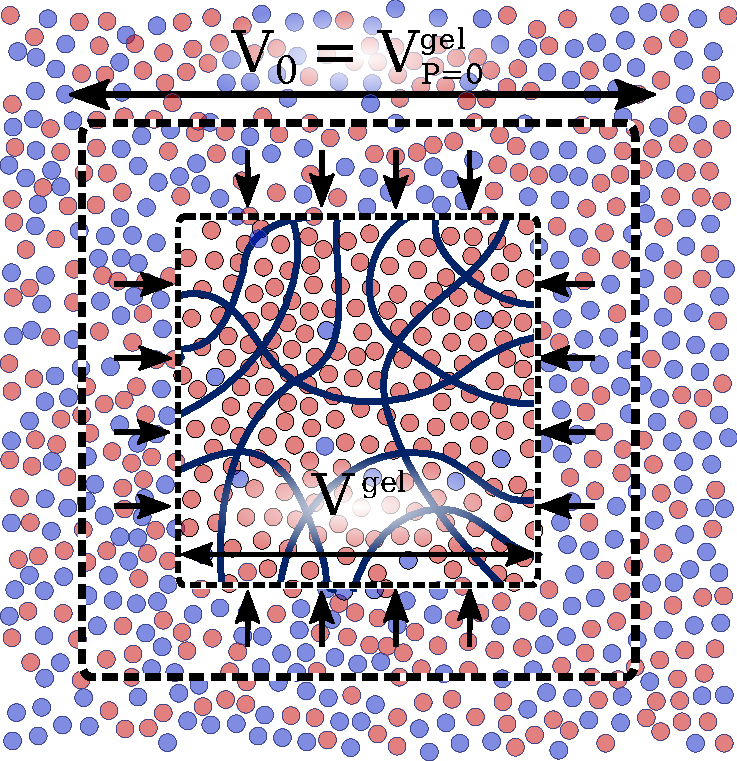
\includegraphics[width=0.5\columnwidth]{{figures/gibbs3}.pdf}}
		\caption{
			Schematic illustration of the hydrogel being compressed isotropically by pressure $\Delta P$ 
			from the initial volume at free swelling equilibrium, $V_0$ to a volume $\Vgel$. 
			Simultaneously, the gel exchanges small ions with a reservoir solution of salinity $\cs$.}
	\end{figure}
\end{frame}

\begin{frame}{Monovalent salt. Desalination effect.}
	\begin{figure}[t]
		\subfloat[low salinity, $c_s = 0.007$ mol/l]
			{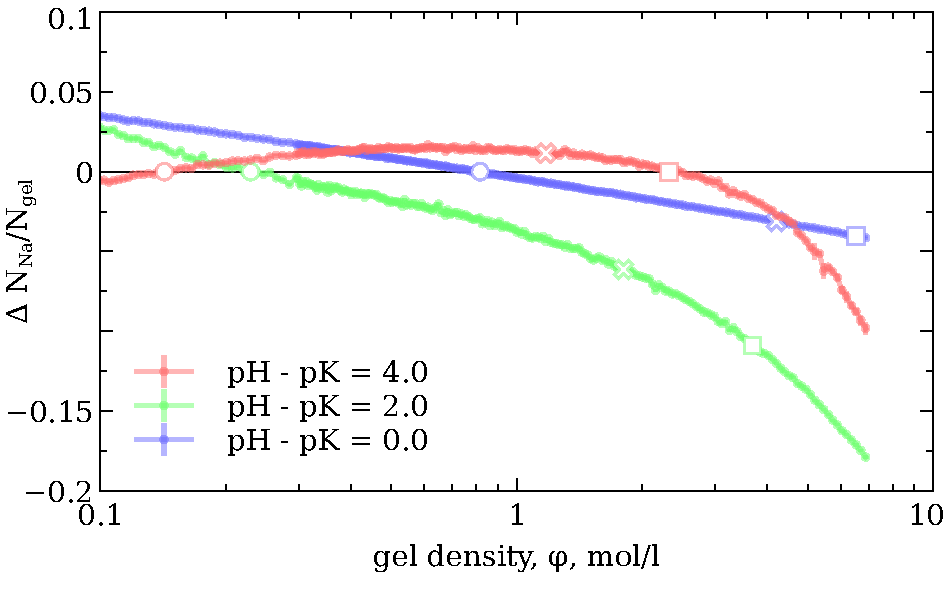
\includegraphics[width=0.5\columnwidth]{{figures/gel_Na_log_density_cs0.006_N_Samples200}.pdf}}
			{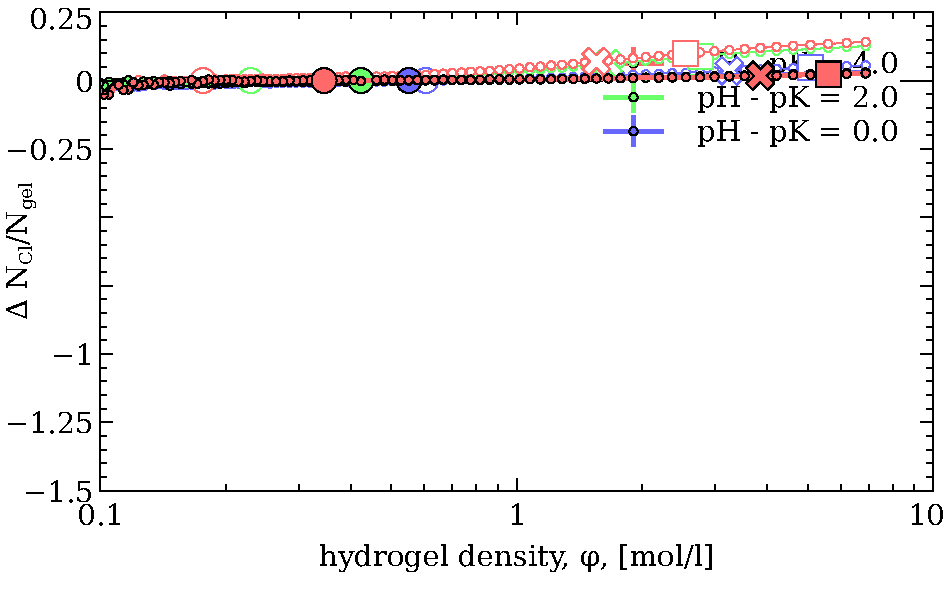
\includegraphics[width=0.5\columnwidth]{{figures/gel_Cl_log_density_cs0.15_N_Samples200}.pdf}}
		\subfloat[high salinity, $c_s = 0.209$ mol/l]
			{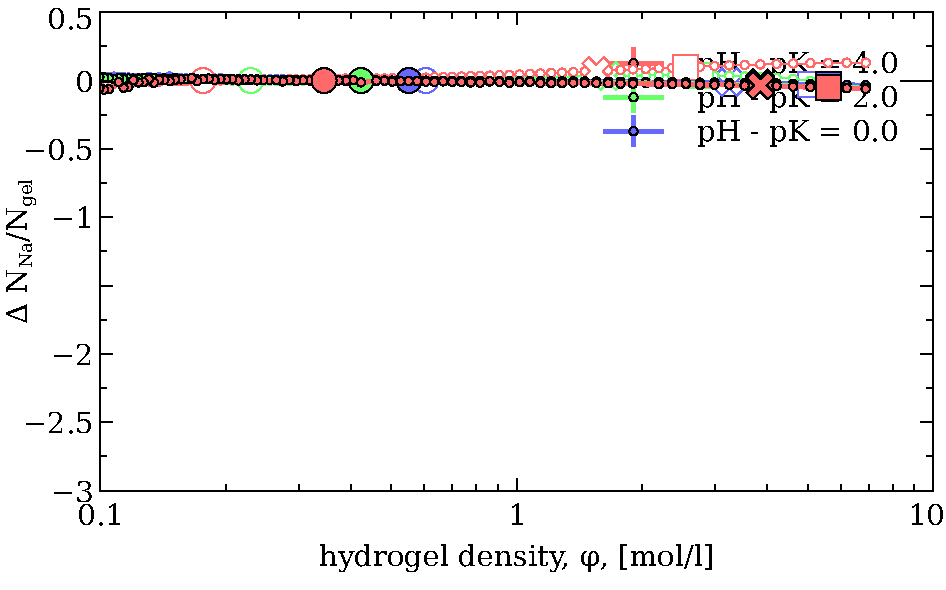
\includegraphics[width=0.5\columnwidth]{{figures/gel_Na_log_density_cs0.15_N_Samples200}.pdf}}
			{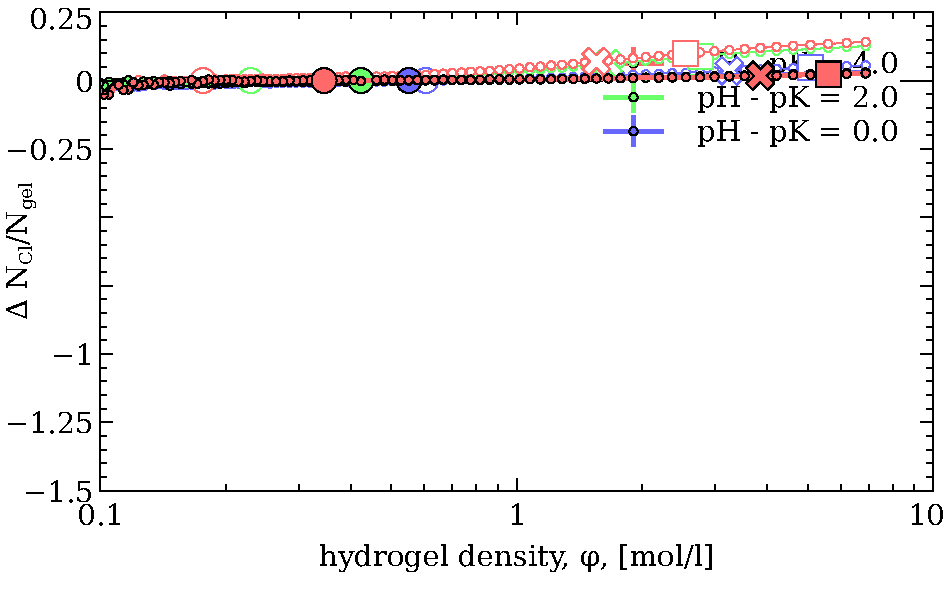
\includegraphics[width=0.5\columnwidth]{{figures/gel_Cl_log_density_cs0.15_N_Samples200}.pdf}}
	\end{figure}
\end{frame}

\begin{frame}{Divalent salt. }
	\begin{columns}[T,onlytextwidth]% COLUMNS
		\column{0.55\textwidth}
			\begin{figure}
				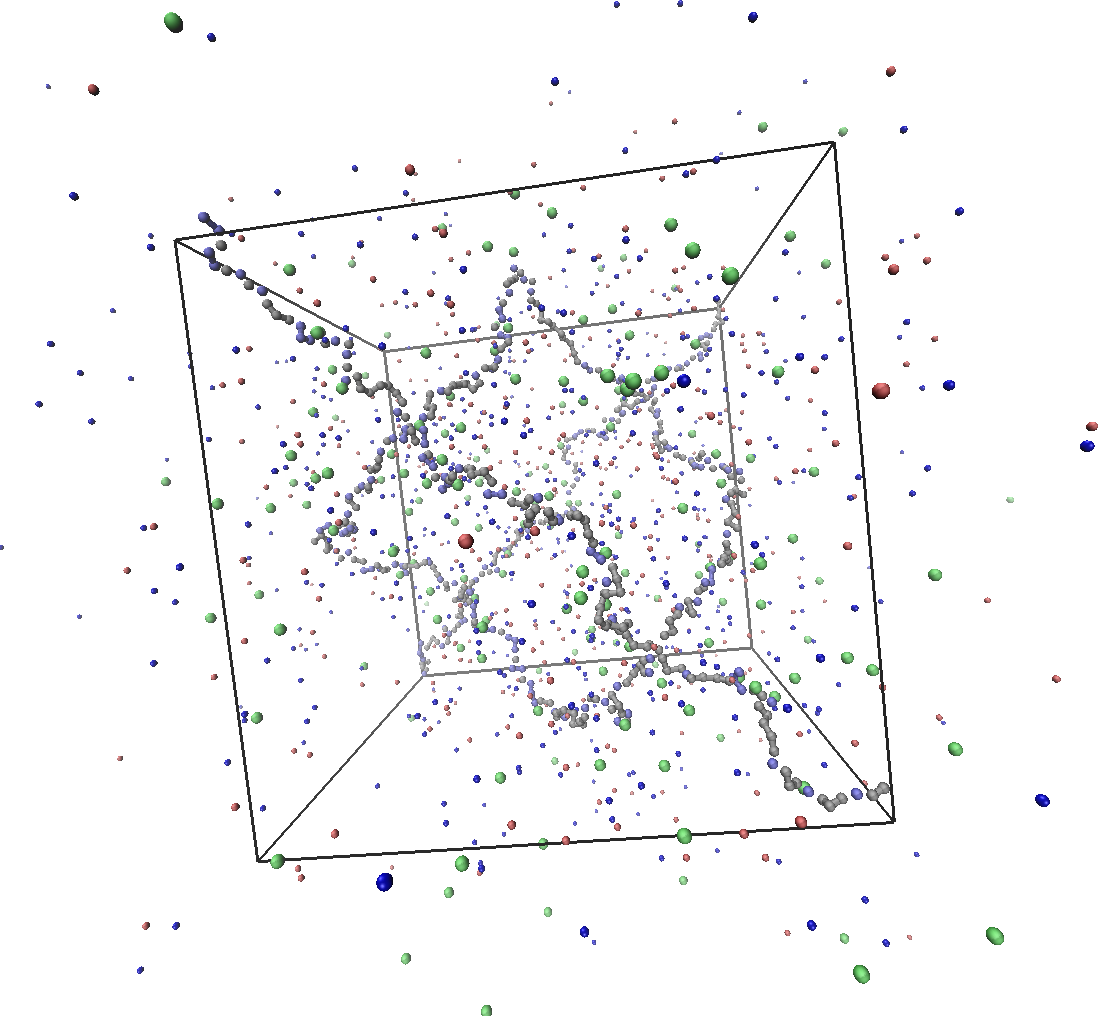
\includegraphics[width=1\columnwidth]{figures/vmdscene.png}
			\end{figure} 		
		\column{0.4\textwidth}
			{\Large Seawater model: }
			\begin{eqnarray*}
				c_\cl&=&0.54\text{ mol/l} \\
				&&\text{of negative ions} 
				%c_\so&=&0.028 \text{ mol/l of negative divalent ions} 
			\end{eqnarray*}
			\begin{eqnarray*}
				c_\na&=&0.47\text{ mol/l} \\
				&&\text{of positive ions} 
			\end{eqnarray*}

			\begin{eqnarray*}
				c_\ca&=&0.063\text{ mol/l} \\
				&&\text{of positive divalent ions}  \\
			\end{eqnarray*}
		
	\end{columns}
	\begin{columns}[T,onlytextwidth]% COLUMNS
		\column{0.5\textwidth}
			\begin{eqnarray*}
				c_{\na}&\simeq0.87\cdot c_{\cl} \\
				c_{\ca}&\simeq0.117\cdot c_{\cl} \\
				%c_{\so}&\simeq&c_{\cl}\cdot0.0282/0.55=0.051c_{\cl} 
			\end{eqnarray*}
		\column{0.5\textwidth}
			\begin{eqnarray*}
				\mu_{\na}&=&\mu_{\cl} - 0.139\kT\\
				\mu_{\ca}&=&\mu_{\cl} - 2.03\kT\\
			\end{eqnarray*}	
	\end{columns}		
\end{frame}
\begin{frame}{Divalent salt. Compression.}



	\begin{figure}[t]
		\subfloat[low salinity, $c_s = 0.007$ mol/l]
			{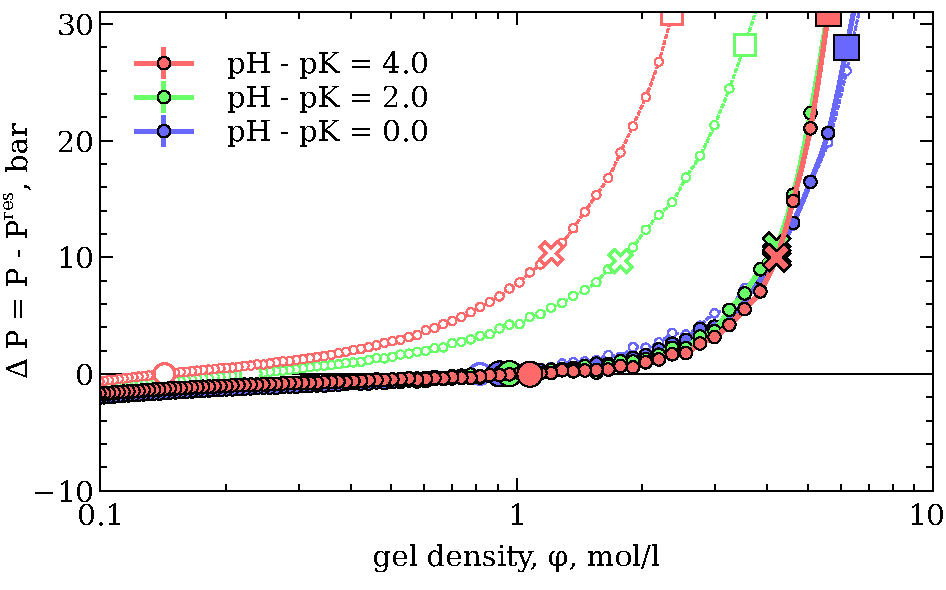
\includegraphics[width=0.5\columnwidth]{{figures/gel_pressure_log_density_pCa3.16_cs0.006_N_Samples200}.pdf}}
			{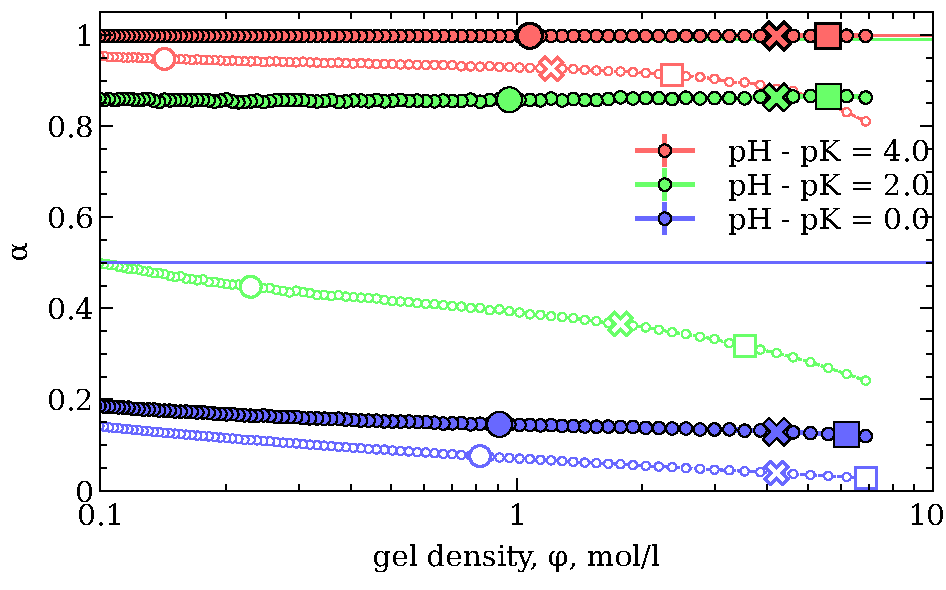
\includegraphics[width=0.5\columnwidth]{{figures/gel_alpha_log_density_pCa3.16_cs0.006_N_Samples200}.pdf}}			
		\subfloat[high salinity, $c_s = 0.209$ mol/l]
			{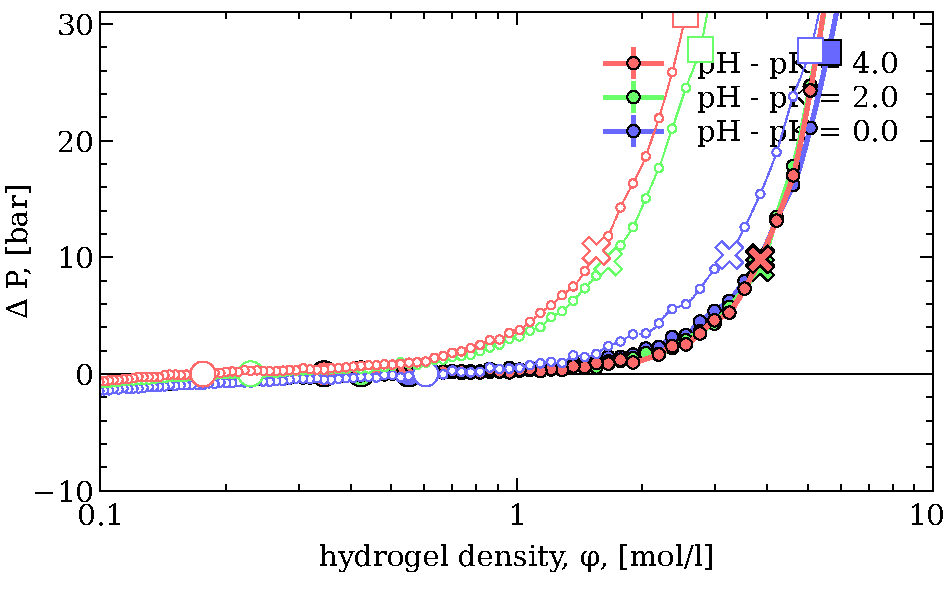
\includegraphics[width=0.5\columnwidth]{{figures/gel_pressure_log_density_pCa1.77_cs0.15_N_Samples200}.pdf}}
			{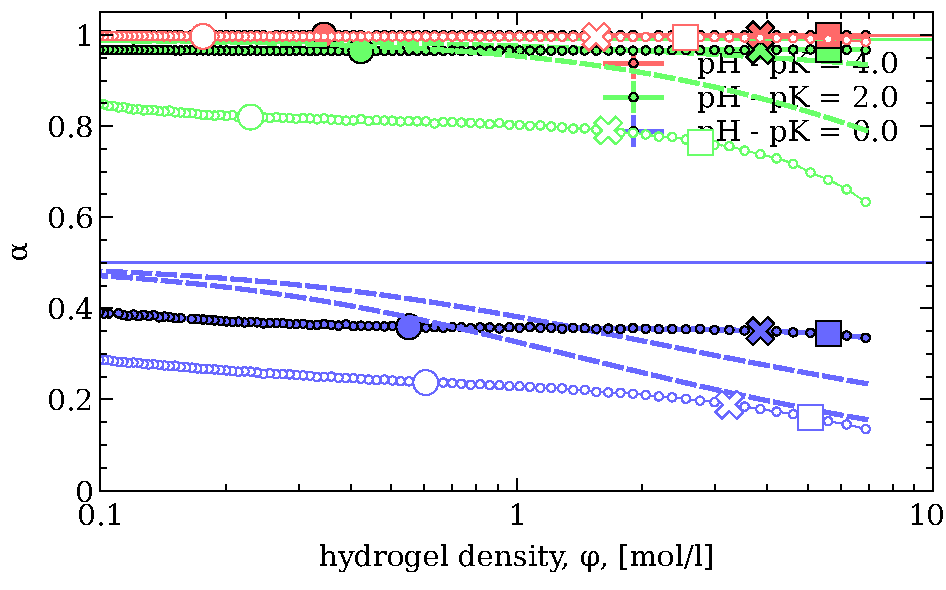
\includegraphics[width=0.5\columnwidth]{{figures/gel_alpha_log_density_pCa1.77_cs0.15_N_Samples200}.pdf}}
	\end{figure}
\end{frame}





\begin{frame}{Divalent salt. Desalination or ion exchange.}
Low salinity $c_\cl = 0.007$
	\begin{figure}
	\subfloat{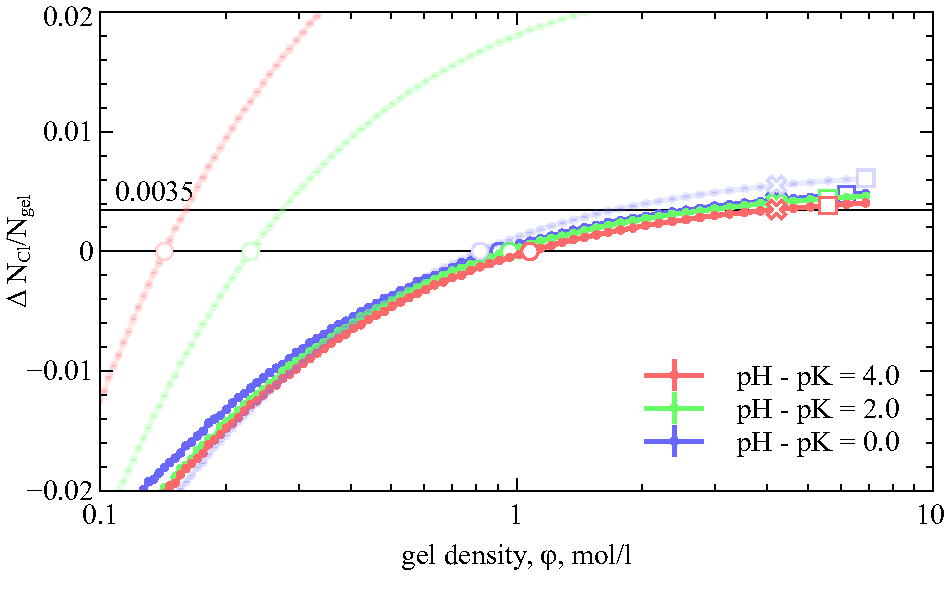
\includegraphics[width=0.5\columnwidth]{{figures/gel_Cl_log_density_pCa3.16_cs0.006_N_Samples200}.pdf}}
	\subfloat{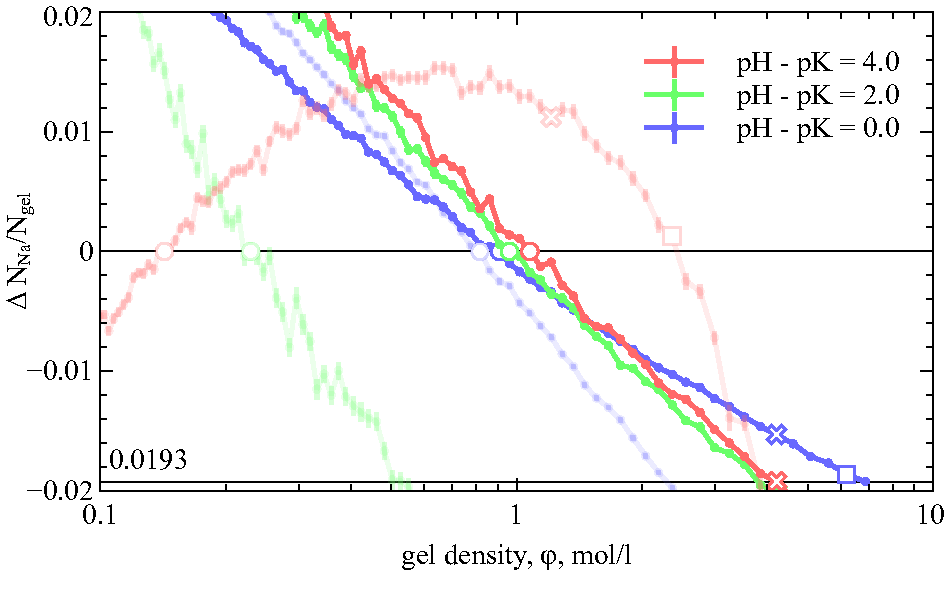
\includegraphics[width=0.5\columnwidth]{{figures/gel_Na_log_density_pCa3.16_cs0.006_N_Samples200}.pdf}}
	\vspace{0.3cm}
	\\
	\subfloat{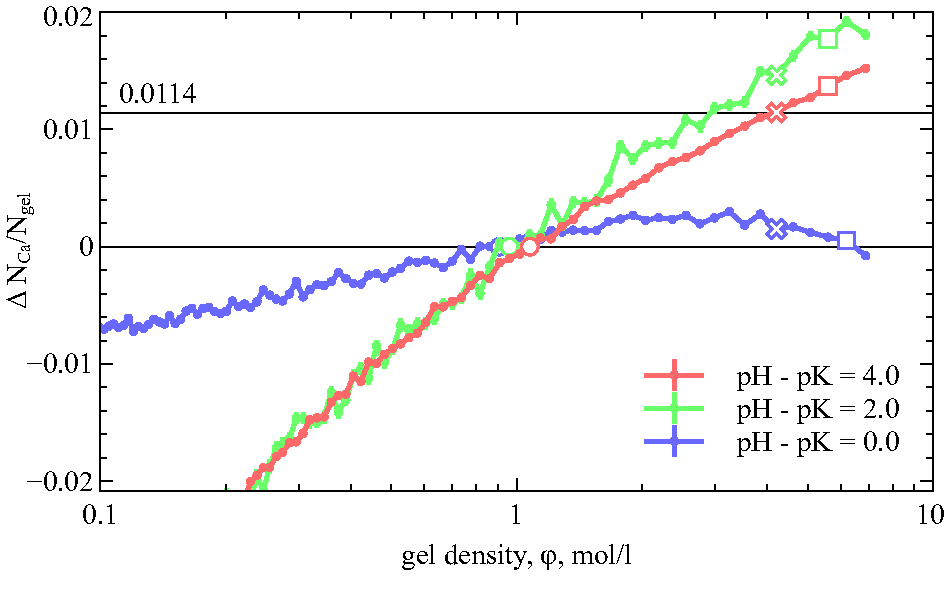
\includegraphics[width=0.5\columnwidth]{{figures/gel_Ca_log_density_pCa3.16_cs0.006_N_Samples200}.pdf}}
	\end{figure}

\end{frame}

\begin{frame}{Divalent salt. Desalination or ion exchange.}
High salinity $c_\cl = 0.263$
	\begin{figure}
	\subfloat{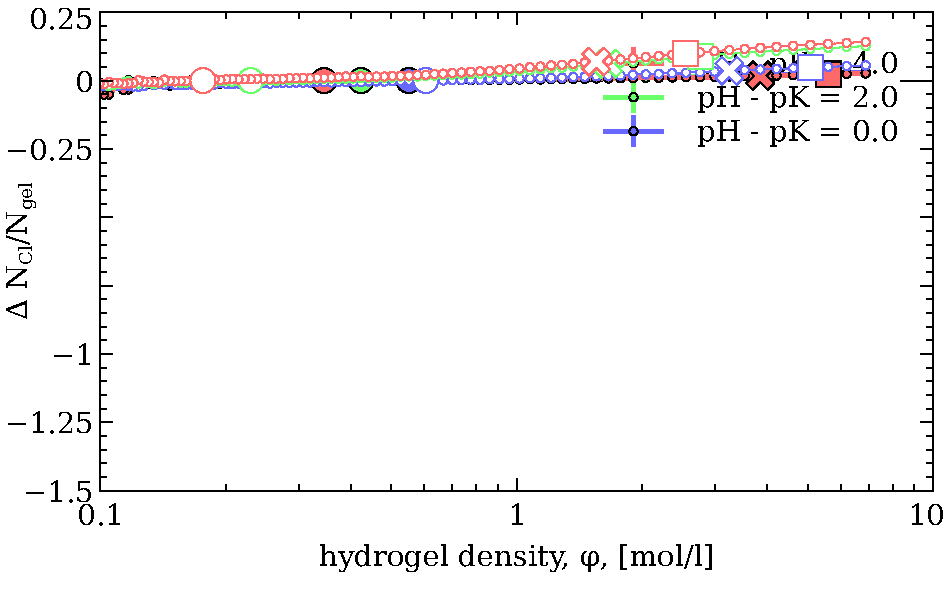
\includegraphics[width=0.5\columnwidth]{{figures/gel_Cl_log_density_pCa1.77_cs0.15_N_Samples200}.pdf}}
	\subfloat{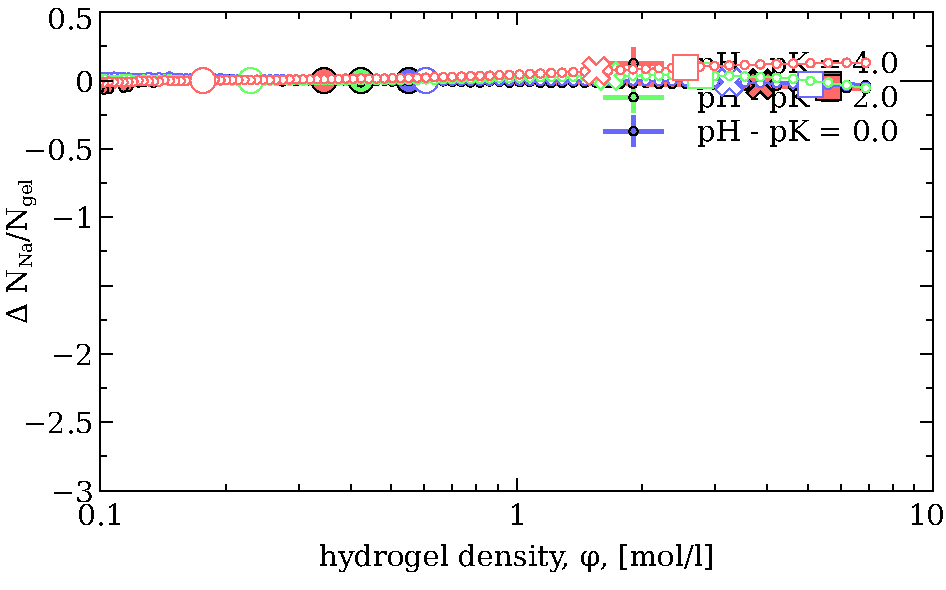
\includegraphics[width=0.5\columnwidth]{{figures/gel_Na_log_density_pCa1.77_cs0.15_N_Samples200}.pdf}}
	\vspace{0.3cm}	
	\\
	\subfloat{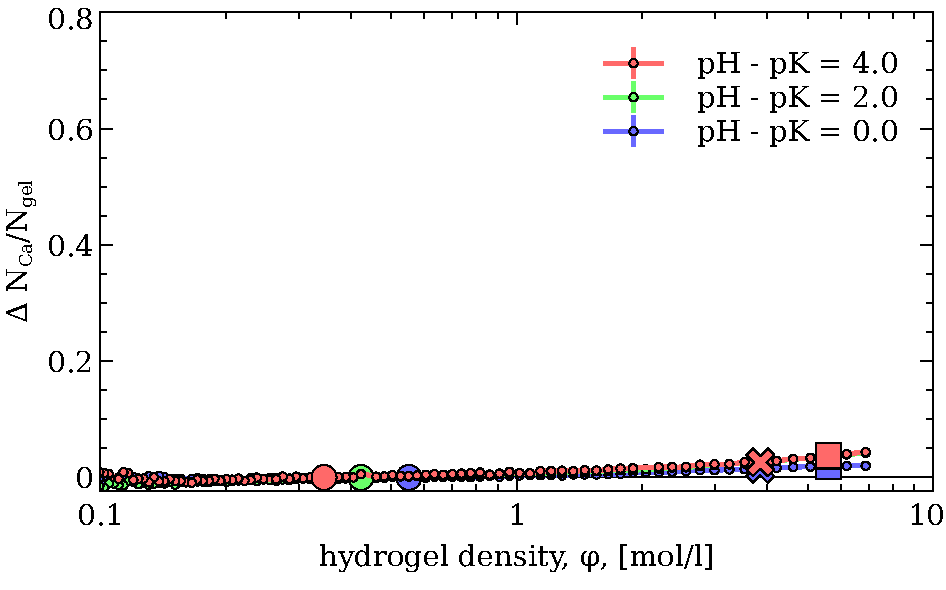
\includegraphics[width=0.5\columnwidth]{{figures/gel_Ca_log_density_pCa1.77_cs0.15_N_Samples200}.pdf}}
	\end{figure}

\end{frame}


\section{Conclusion}

\begin{frame}{Summary}
\begin{enumerate}
\item monovalent ions
	\begin{enumerate}
		\item ionization of the hydrogel is suppressed as compared to predictions for monomeric acid, due 
			\begin{itemize}
				\item to the Donnan partitioning of H + ions; 
				\item to the electrostatic repulsion between charges of the gel.
			\end{itemize}
		\item the decrease of ionisation degree is much less significant than previously estimated using mean-feld models.
		\item decreasing the ionization of the gel upon compression may completely reverse the desalination effect forcing the gel to  release counterions upon compression instead of absorbing them.
	\end{enumerate}
\item with divalent ions
	\begin{enumerate}
		\item the electrostatics is almost completelly screened
		\item alpha does not change versus compression
		\item The compression of gel in presence of divalent ions works as ion exchanger of Ca ion by Na
	\end{enumerate}
\end{enumerate}
\end{frame}

{\setbeamercolor{palette primary}{fg=black, bg=yellow}
\begin{frame}[standout]
  Questions?
\end{frame}
}

\appendix


\begin{frame}{Monovalent salt. ``No electrostatics'' vs ``Mean field theory''.}
	\begin{figure}[t]
		\subfloat[low salinity, $c_s = 0.007$ mol/l]
			{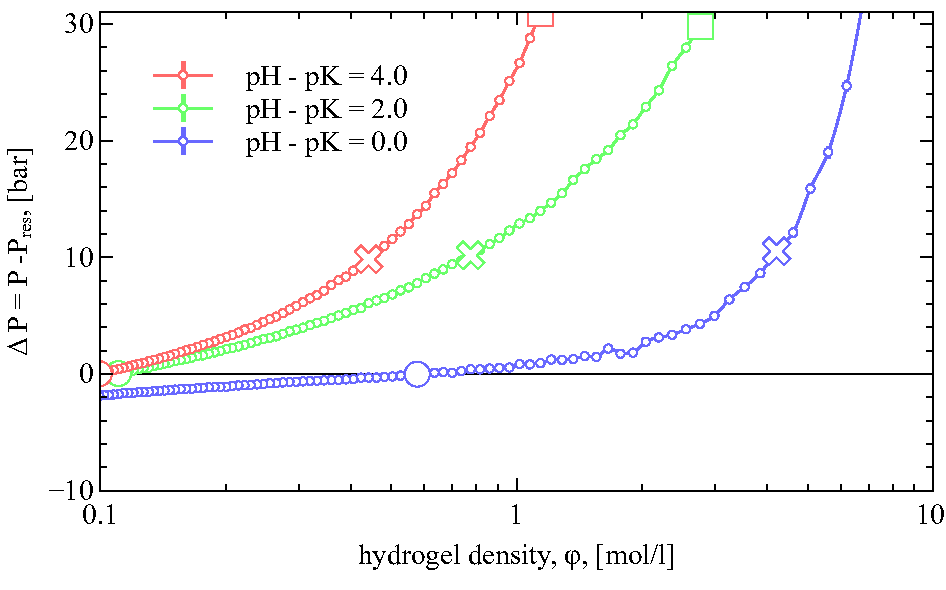
\includegraphics[width=0.5\columnwidth]{{figures/gel_pressure_log_density_lB0.0_cs0.006_N_Samples200}.pdf}}
			{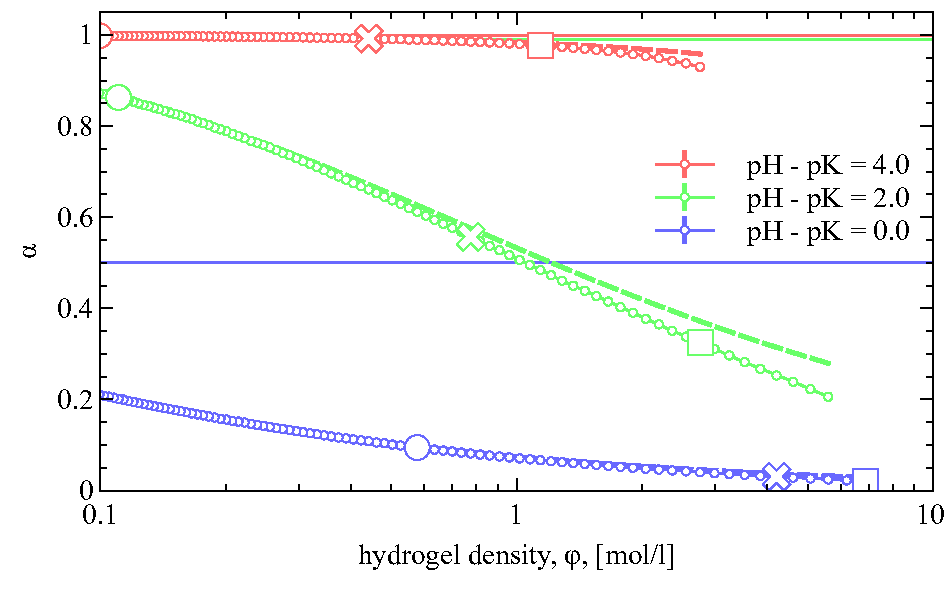
\includegraphics[width=0.5\columnwidth]{{figures/gel_alpha_log_density_lB0.0_cs0.006_N_Samples200}.pdf}}
		\subfloat[high salinity, $c_s = 0.209$ mol/l]
			{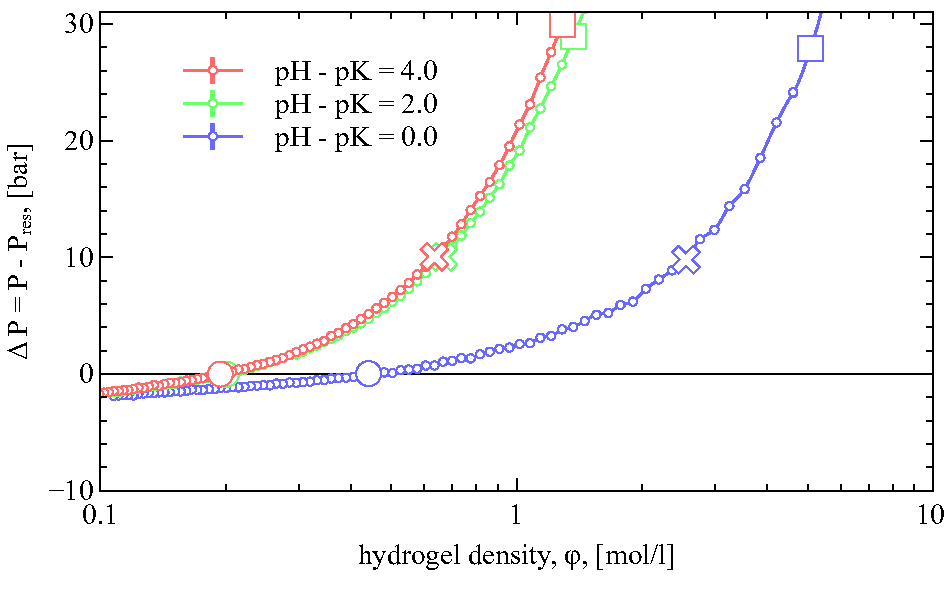
\includegraphics[width=0.5\columnwidth]{{figures/gel_pressure_log_density_lB0.0_cs0.15_N_Samples200}.pdf}}
			{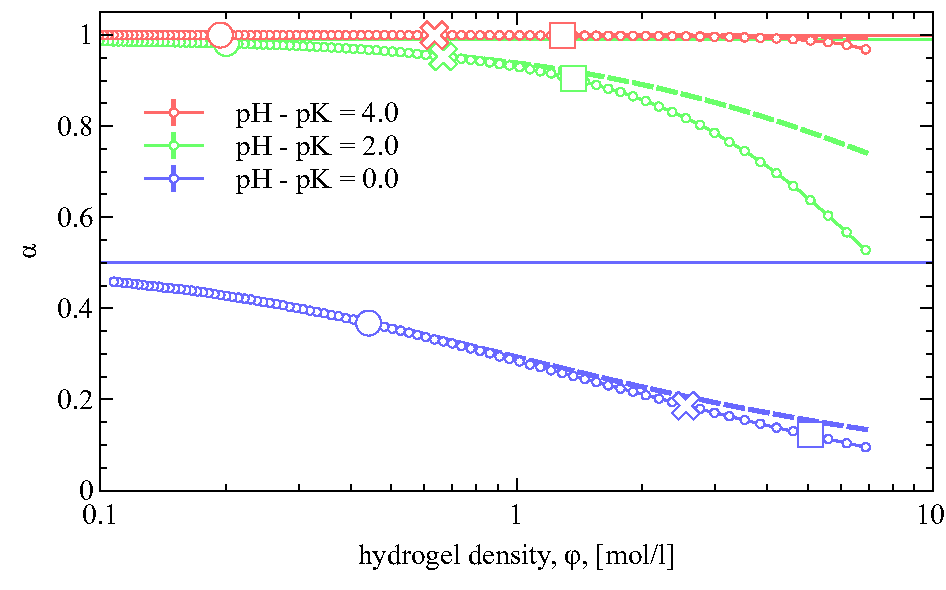
\includegraphics[width=0.5\columnwidth]{{figures/gel_alpha_log_density_lB0.0_cs0.15_N_Samples200}.pdf}}
	\end{figure}
\end{frame}
\end{document}
\begin{frame}[fragile]{Typography}
      \begin{verbatim}The theme provides sensible defaults to
\emph{emphasize} text, \alert{accent} parts
or show \textbf{bold} results.\end{verbatim}

  \begin{center}becomes\end{center}

  The theme provides sensible defaults to \emph{emphasize} text,
  \alert{accent} parts or show \textbf{bold} results.
\end{frame}

\begin{frame}{Font feature test}
  \begin{itemize}
    \item Regular
    \item \textit{Italic}
    \item \textsc{SmallCaps}
    \item \textbf{Bold}
    \item \textbf{\textit{Bold Italic}}
    \item \textbf{\textsc{Bold SmallCaps}}
    \item \texttt{Monospace}
    \item \texttt{\textit{Monospace Italic}}
    \item \texttt{\textbf{Monospace Bold}}
    \item \texttt{\textbf{\textit{Monospace Bold Italic}}}
  \end{itemize}
\end{frame}

\begin{frame}{Lists}
  \begin{columns}[T,onlytextwidth]% COLUMNS
    \column{0.33\textwidth}
      Items
      \begin{itemize}
        \item Milk \item Eggs \item Potatos
      \end{itemize}

    \column{0.33\textwidth}
      Enumerations
      \begin{enumerate}
        \item First, \item Second and \item Last.
      \end{enumerate}

    \column{0.33\textwidth}
      Descriptions
      \begin{description}
        \item[PowerPoint] Meeh. \item[Beamer] Yeeeha.
      \end{description}
  \end{columns}
\end{frame}
\begin{frame}{Animation}
  \begin{itemize}[<+- | alert@+>]
    \item \alert<4>{This is\only<4>{ really} important}
    \item Now this
    \item And now this
  \end{itemize}
\end{frame}
\begin{frame}{Figures}
  \begin{figure}
    \newcounter{density}
    \setcounter{density}{20}
    \begin{tikzpicture}
      \def\couleur{alerted text.fg}
      \path[coordinate] (0,0)  coordinate(A)
                  ++( 90:5cm) coordinate(B)
                  ++(0:5cm) coordinate(C)
                  ++(-90:5cm) coordinate(D);
      \draw[fill=\couleur!\thedensity] (A) -- (B) -- (C) --(D) -- cycle;
      \foreach \x in {1,...,40}{%
          \pgfmathsetcounter{density}{\thedensity+20}
          \setcounter{density}{\thedensity}
          \path[coordinate] coordinate(X) at (A){};
          \path[coordinate] (A) -- (B) coordinate[pos=.10](A)
                              -- (C) coordinate[pos=.10](B)
                              -- (D) coordinate[pos=.10](C)
                              -- (X) coordinate[pos=.10](D);
          \draw[fill=\couleur!\thedensity] (A)--(B)--(C)-- (D) -- cycle;
      }
    \end{tikzpicture}
    \caption{Rotated square from
    \href{http://www.texample.net/tikz/examples/rotated-polygons/}{texample.net}.}
  \end{figure}
\end{frame}
\begin{frame}{Tables}
  \begin{table}
    \caption{Largest cities in the world (source: Wikipedia)}
    \begin{tabular}{lr}
      \toprule
      City & Population\\
      \midrule
      Mexico City & 20,116,842\\
      Shanghai & 19,210,000\\
      Peking & 15,796,450\\
      Istanbul & 14,160,467\\
      \bottomrule
    \end{tabular}
  \end{table}
\end{frame}
\begin{frame}{Blocks}
  Three different block environments are pre-defined and may be styled with an
  optional background color.

  \begin{columns}[T,onlytextwidth]% COLUMNS
    \column{0.5\textwidth}
      \begin{block}{Default}
        Block content.
      \end{block}

      \begin{alertblock}{Alert}
        Block content.
      \end{alertblock}

      \begin{exampleblock}{Example}
        Block content.
      \end{exampleblock}

    \column{0.5\textwidth}

      \metroset{block=fill}

      \begin{block}{Default}
        Block content.
      \end{block}

      \begin{alertblock}{Alert}
        Block content.
      \end{alertblock}

      \begin{exampleblock}{Example}
        Block content.
      \end{exampleblock}

  \end{columns}% COLUMNS
\end{frame}
\begin{frame}{Math}
  \begin{equation*}
    e = \lim_{n\to \infty} \left(1 + \frac{1}{n}\right)^n
  \end{equation*}
\end{frame}
\begin{frame}{Line plots}
  \begin{figure}
    \begin{tikzpicture}
      \begin{axis}[
        mlineplot,
        width=0.9\textwidth,
        height=6cm,
      ]

        \addplot {sin(deg(x))};
        \addplot+[samples=100] {sin(deg(2*x))};

      \end{axis}
    \end{tikzpicture}
  \end{figure}
\end{frame}
\begin{frame}{Bar charts}
  \begin{figure}
    \begin{tikzpicture}
      \begin{axis}[
        mbarplot,
        xlabel={Foo},
        ylabel={Bar},
        width=0.9\textwidth,
        height=6cm,
      ]

      \addplot plot coordinates {(1, 20) (2, 25) (3, 22.4) (4, 12.4)};
      \addplot plot coordinates {(1, 18) (2, 24) (3, 23.5) (4, 13.2)};
      \addplot plot coordinates {(1, 10) (2, 19) (3, 25) (4, 15.2)};

      \legend{lorem, ipsum, dolor}

      \end{axis}
    \end{tikzpicture}
  \end{figure}
\end{frame}
\begin{frame}{Quotes}
  \begin{quote}
    Veni, Vidi, Vici
  \end{quote}
\end{frame}

{%
\setbeamertemplate{frame footer}{My custom footer}
\begin{frame}[fragile]{Frame footer}
    \themename defines a custom beamer template to add a text to the footer. It can be set via
    \begin{verbatim}\setbeamertemplate{frame footer}{My custom footer}\end{verbatim}
\end{frame}
}

\begin{frame}{References}
  Some references to showcase [allowframebreaks] \cite{knuth92,ConcreteMath,Simpson,Er01,greenwade93}
\end{frame}

\section{Conclusion}

\begin{frame}{Summary}

  Get the source of this theme and the demo presentation from

  \begin{center}\url{github.com/matze/mtheme}\end{center}

  The theme \emph{itself} is licensed under a
  \href{http://creativecommons.org/licenses/by-sa/4.0/}{Creative Commons
  Attribution-ShareAlike 4.0 International License}.

  \begin{center}\ccbysa\end{center}

\end{frame}

{\setbeamercolor{palette primary}{fg=black, bg=yellow}
\begin{frame}[standout]
  Questions?
\end{frame}
}

\appendix

\begin{frame}[fragile]{Backup slides}
  Sometimes, it is useful to add slides at the end of your presentation to
  refer to during audience questions.

  The best way to do this is to include the \verb|appendixnumberbeamer|
  package in your preamble and call \verb|\appendix| before your backup slides.

  \themename will automatically turn off slide numbering and progress bars for
  slides in the appendix.
\end{frame}

\begin{frame}[allowframebreaks]{References}

  \bibliography{hydrogel}
  \bibliographystyle{abbrv}

\end{frame}

